% Capítulo 2
\chapter{Estado da Arte}
\label{Capitulo2}

\begin{flushright}
\textit{```You are entering a world of pain.''} \\[0.5em]
--- Walter Sobchak, \textit{The Big Lebowski}
\end{flushright}

Tendo em conta a nossa experiência como professor numa escola secundária, neste capítulo procuramos  fazer o enquadramento das principais dificuldades que a Educação (digital) atravessa em Portugal e discutir em que medida a integração da tecnologia digital na educação é essencial para criar ambientes de aprendizagem mais eficazes e adaptados à evolução do panorama digital. Explora-se o potencial de tecnologias, como os laboratórios remotos, para o desenvolvimento de experiências de aprendizagem personalizadas e reflete-se sobre a forma como podem ajudar a suprir estas mesmas dificuldades.
Face a isto, discute-se a ascensão do \textit{eLearning}, particularmente no contexto da abordagem \acrshort{stem}, assim como a evolução da educação das salas de aula tradicionais para ambientes virtuais, enfatizando as oportunidades e possibilidades de aprendizagem alargadas oferecidas pelo \textit{eLearning}

\section{Transformação digital na educação}
\label{sec:transformaçãodigital}

\colorbox{yellow}{\textbf{NOTA:} O prof sugeriu que os pontos 2.1 e 2.2 pudessem ficar num só ponto}

\colorbox{yellow}{ no entanto, parece-me fazer sentido que fiquem separados, se calhar depois do}

\colorbox{yellow}{prof ler possa ter outra percepção. Deixo para consideração depois de ler.}

A educação está a sofrer grandes mudanças a nível tecnológico, social e humano. Estas foram impulsionadas pela pandemia \acrfull{covid-19}, que expôs as fragilidades em termos de gestão e capacitação dos recursos tecnológicos e do eLearning\footnote{Jay Cross, é conhecido por ter ``cunhado'' pela primeira vez o termo \textit{eLearning}\cite{jaycross}. Por isso, nesta tese, o termo será sempre referido desta forma, em vez de \textit{e-Learning}}. O sistema educativo português está longe da perfeição (ou, se nos atrevermos a dizê-lo, está longe de ser razoável) mas, durante a pandemia, devido a um grande esforço coletivo, respondeu imediatamente a este enorme obstáculo. Num curto espaço de tempo, o ensino presencial e o contacto humano foram substituídos pelo ensino à distância.

\textbf{Estávamos pronto para isto?}

Antes da pandemia, no Ensino Básico, as tecnologias digitais eram mais frequentemente utilizadas como meio de comunicação do que como ferramenta pedagógica \cite{oecd_using_2021}. Nas últimas duas décadas aproximadamente, Portugal já introduziu programas para abordar a digitalização na educação. O programa de digitalização contemplado no Plano de Ação para a Transição Digital (Resolução do Conselho de Ministros n.º 30/2020, de 21 de abril) prevê, entre outras medidas, uma forte aposta na formação digital dos professores, no desenvolvimento digital das escolas e na disponibilização de recursos educativos digitais \cite{transicaodigital} \cite{capacitacaodigital}.

No mundo de hoje, cada vez mais digital, 3.6 mil milhões de pessoas ainda não têm acesso à \textit{Internet}\cite{TheDigitransf}. Este problema reduz o acesso a um mundo de informações disponíveis \textit{online} e limita o potencial de aprendizagem e crescimento, para não falar das competências digitais de que as pessoas necessitam para aprender e melhorar as suas vidas.
A crise da \acrshort{covid-19} mostrou-nos como a ligação à \textit{Internet} é crucial para as actividades quotidianas, como o trabalho e a aprendizagem. Hoje, mais do que nunca, é necessário reforçar as infra-estruturas nacionais para garantir que a conetividade esteja mais amplamente disponível. Igualmente importante é reforçar os planos de conetividade das escolas e investir numa aprendizagem de qualidade, a fim de melhorar o acesso à educação, os resultados da aprendizagem e o potencial de ganhos dos jovens, bem como o desenvolvimento socioeconómico das suas comunidades e países \cite{TheDigitransf}.
Se adoptarmos uma abordagem geral da integração da tecnologia digital \cite{DESI2020}, Portugal ocupa o 19º lugar entre os 28  Estados-Membros da \acrfull{ue} no \acrfull{desi} 2020.
Apesar de alguns progressos na dimensão do capital humano, graças a uma melhoria do nível básico de competências digitais e a uma maior percentagem de diplomados em \acrfull{tic}, este aspeto continua a ser particularmente crítico para Portugal, dado o atual baixo nível de literacia digital da sua população.

Relativamente à dimensão capital humano, Portugal ocupa o 21º lugar entre 28 países da \acrshort{ue} - uma melhoria de dois lugares em relação ao ano anterior, mas ainda abaixo da média da \acrshort{ue}. Em 2019, a percentagem da população portuguesa sem, pelo menos, competências digitais básicas diminuiu de 50\% para 48\%. \textcolor{red}{\textbf{REVER ESTA AFIRMAÇÃO}}
No entanto, cerca de 26\% dos cidadãos portugueses não tinham quaisquer competências digitais. Isto deve-se principalmente ao facto de muitas pessoas nunca terem utilizado a Internet \cite{DESI2020}.

Podemos deduzir que esta realidade está relacionada com os baixos níveis de educação que ainda existem no país. No entanto, há outros factores que são visíveis para todos, como o elevado preço dos serviços de \textit{Internet} ou o baixo número de licenciados em \acrshort{tic}: ``A proporção de especialistas em \acrshort{tic} representa uma percentagem menor da força de trabalho em comparação com a média da \acrshort{ue} (2,4\% contra 3,9\% na \acrshort{ue}). Além disso, Portugal continua a ter uma das mais baixas percentagens de especialistas de \acrshort{tic} no emprego feminino total, representando metade da média da \acrshort{ue}. A proporção de licenciados em \acrshort{tic} no total de licenciados melhorou, mas é ainda muito baixa para os padrões da \acrshort{ue} (1,9\% em comparação com 3,6\% na \acrshort{ue})'' \cite{DESI2020}.
Esta falta de competências básicas foi agravada pela pandemia. De acordo com o relatório \textit{``Juventude e COVID 19: impactos no emprego, na educação, nos direitos e no bem-estar mental''} \cite{impactocovideducacao}, 65\% consideram que aprenderam menos desde o início da pandemia devido à transição das aulas presenciais para as aulas \textit{online} durante o confinamento. Apesar dos seus esforços para continuar a estudar, metade destes jovens acredita que os seus estudos vão ficar para trás e 9\% pensa que podem reprovar devido a estas dificuldades. A situação foi pior para os jovens que vivem em países de baixos rendimentos, por haver menos acesso à \textit{Internet}, uma falta crítica de equipamentos, e às vezes nenhum lugar em casa para a aprendizagem adequada \cite{impactocovideducacao}.

Com base nestes resultados, o estudo conclui que ``os desafios colocados pela transição para o ensino fora da sala de aula e em casa'' foram enormes. Mesmo quando as instituições conseguiram fazer a transição para a aprendizagem \textit{online}, os professores, formadores e estudantes podem não ter tido a capacidade de ``garantir a continuidade da aprendizagem''. Entre os factores que dificultam a eficácia do ensino \textit{online} contam, como já foi referido: baixos níveis de acesso à \textit{Internet}; lacunas nas competências digitais; incapacidade de ensinar e aprender à distância; falta de equipamento informático em casa; falta de espaço; falta de materiais preparados para o \textit{eLearning}; e falta de trabalho de grupo e de contacto social - ambos componentes fundamentais do processo de aprendizagem.

Como professor do ensino secundário e director de turma, que tinha de lidar tanto com professores como com alunos, pudemos observar estes problemas do lado dos alunos, principalmente: não terem computador portátil ou pessoal, não terem acesso à \textit{internet} ou esta ser lenta. Houve mesmo alguns casos de alunos que tiveram de assistir às aulas através do telemóvel. Do lado dos professores, esperava-se um enorme desafio, principalmente devido à falta de experiência na leccionação \textit{online} e às dificuldades em encontrar e utilizar as várias ferramentas \textit{online}. A ``curva de aprendizagem'' foi muito lenta.

Obviamente, não só em Portugal, mas também em todo o mundo, as escolas e instituições encerraram em meados de março de 2020 e os alunos de todos os níveis de ensino assistiram às aulas e interagiram com os professores através de videoconferências e outras ferramentas \textit{online}. A \acrfull{unesco} apoiou a implementação de programas de ensino à distância em grande escala e recomendou aplicações e plataformas educativas gratuitas que as escolas e os professores poderiam utilizar para comunicar com os alunos à distância. A organização partilhou depois as melhores práticas para tirar partido de tecnologias móveis pouco dispendiosas para fins de ensino e aprendizagem, a fim de atenuar as perturbações no ensino \cite{unesco}.

O \acrfull{prr} recomenda a entrega de computadores portáteis a todos os alunos e professores do ensino primário e secundário. Supostamente deveriam ter sido entregues 600 mil computadores (com acesso à Internet), mas ainda há um longo caminho a percorrer. Em agosto de 2022, apenas 70\% desses computadores tinham chegado aos utilizadores. A principal razão? Os pais foram confrontados com o compromisso de reembolsar o dinheiro investido pelo Estado ,se não pudessem devolvê-los nas mesmas condições em que os tinham recebido\cite{entregacomputadores}.

Entretanto, \colorbox{yellow}{\textbf{REFERIR AQUI CASO PESSOAL EM CONTEXTO }}

\colorbox{yellow}{\textbf{DE SALA DE AULA??? - OPINIÃO PROF}} as aulas de laboratório (electrónica) eram as que menos sentido faziam: por exemplo, o contacto com uma placa branca - também conhecida por \textit{breadboard} ou placa de ensaio - e todos os componentes físicos foi substituído pelo recurso a dois simuladores online: \href{https://www.multisim.com/}{\textbf{Multisim}} e \href{https://www.falstad.com/circuit/}{\textbf{Falstad}}.
Felizmente, estes já eram utilizados na sala de aula, embora como complemento da vertente mais prática do ensino.

\vspace{1cm}
Assim, a resposta à questão colocada anteriormente é: \textbf{não}.
\vspace{1cm}

Ninguém estava preparado para estas mudanças nem para o ensino \textit{online} e o \textit{eLearning}.

Como já foi referido, os desafios para alunos e professores foram enormes, a adaptação ao ensino/aprendizagem \textit{online} teve de ser feita muito rapidamente e os recursos digitais tornaram-se a ``tábua de salvação'' da educação. No entanto, as oportunidades que as tecnologias digitais oferecem vão muito além do apoio de emergência utilizado durante a pandemia.
Atualmente, está disponível um número infinito de possibilidades, novas respostas para o quê, como e quando as pessoas aprendem \cite{oecd_state_2021}.

A forma de pensar dos estudantes de hoje é também muito diferente da de há trinta anos. De uma forma mais particular, o pensamento mudou muito desde que a \textit{Internet} e os recursos digitais começaram a tornar-se massivos.
É essencial que os alunos possam aceder à tecnologia e utilizá-la para se desenvolverem ainda mais e a lição mais importante de todas é: \textbf{permitir-lhes compreender o que fazer com a informação e os recursos que estão à sua disposição de tantas formas diferentes}.
Esta nova adaptação educativa (ou deveríamos chamar-lhe ``evolução''?) ``também adapta a aprendizagem aos estilos de aprendizagem pessoais com uma granularidade e precisão muito maiores do que qualquer ambiente de sala de aula tradicional pode fazer. Do mesmo modo, \textbf{laboratórios virtuais} dão aos alunos a oportunidade de conceber, realizar e aprender com as experiências, em vez de se limitarem a aprender sobre elas'' \cite{oecd_state_2021}.

Em agosto de 2020, numa citação incluída num artigo publicado no \textit{Diário de Notícias}, um aluno afirmava:
\begin{center}
    \textbf{``As aulas de laboratório foram as que menos sentido fizeram para mim, pois fazer relatórios e cálculos sobre experiências que não fizemos, sem adquirir/desenvolver as competências e técnicas que é suposto esta componente da disciplina nos dar, é um pouco ridículo.}'' \cite{impactonegativocovid}.
\end{center}

Por outro lado, os professores devem desenvolver a sua literacia digital, para melhor dominarem estas novas ferramentas na sala de aula, de forma a ajudarem os alunos a construírem o seu próprio conhecimento.

Assim, é evidente que a Educação, como um todo, precisa de se inserir neste contexto que está cada vez mais presente no quotidiano de todos.

O mundo é cada vez mais dominado pela tecnologia (... e nestes tempos actuais começa o domínio da Inteligência Artificial), milhares de milhões de dispositivos físicos em todo o mundo estão agora ligados à \textit{Internet}, todos recolhendo e partilhando dados. Atualmente, os \textit{chips} de computador são muito baratos e a ubiquidade das redes sem fios permite ligar qualquer coisa, desde algo tão pequeno como um comprimido até algo tão grande como um avião. É o que se designa por \acrfull{iot} \cite{IoT}.
Por conseguinte, a informação e os recursos estão ``na ponta dos dedos de todos'' e à distância de um clique.

\begin{center}
    {\textit{Chegou o momento de os países aproveitarem as lições da pandemia para reconfigurarem as pessoas, os espaços, o tempo e a tecnologia, de modo a criarem ambientes educativos mais eficazes e eficientes}} \cite{thestateofeducation}.
\end{center}

\section{Educação Digital em Portugal: Avanços e Desafios}
\label{sec:educacaodigital}	%For referencing the chapter elsewhere, use \ref{educacaodigital} 

Nos últimos anos, é evidente que estamos a enfrentar grandes mudanças tecnológicas. Os conhecimentos e as competências têm de acompanhar esta evolução. (Este facto ficou bem patente com a pandemia\ldots).

Praticamente todas as aprendizagens e futuros empregos exigirão um certo nível de competências e aptidões digitais. A constante evolução tecnológica exige o desenvolvimento de competências ao longo da vida\cite{Digitale13:online}.
No entanto, em média, dois em cada cinco europeus com idades compreendidas entre os 16 e os 74 anos ainda não possuem estas competências\cite{DESI2020}.

Se reflectirmos sobre esta ideia em contexto educativo e acrescentarmos o facto de o ensino da eletrónica em Portugal passar pelo ensino profissional \textbf{\textcolor{red}{ACHO QUE NÃO REFERI!! - A REVER}}, como já foi referido anteriormente, e se o objetivo é a evolução e inovação no processo de ensino/aprendizagem, é necessário proporcionar a todos os intervenientes as condições e ferramentas necessárias para que o trabalho possa ser desenvolvido e, consequentemente, os alunos realmente aprendam.

A evolução da educação digital em Portugal pode ser aferida pelas crescentes iniciativas governamentais e adopção de tecnologias digitais nas escolas e universidades. Nos últimos anos, Portugal tem investido significativamente na educação digital, reconhecendo a importância das competências digitais para o futuro dos seus cidadãos e a competitividade do país. Este esforço é materializado através de várias iniciativas e programas governamentais que visam integrar a tecnologia no sistema educacional, capacitar professores e preparar os estudantes para a era digital. As medidas de apoio aos objetivos digitais representam um montante que corresponde a 22\% da dotação total do plano, ultrapassando o limiar de 20\% definido pela regulamentação europeia \cite{Transicaodigitalprr}. \sout{: 12 das 20 componentes do \acrshort{prr} têm contributo direto meta digital .}

Lançado em 2017, o Plano Nacional de Competências Digitais (INCoDe.2030)\cite{incode2030} é uma iniciativa ambiciosa do governo português para aumentar a literacia digital de toda a população. Este plano está estruturado em cinco eixos principais: inclusão, educação, qualificação, especialização e investigação.
Como complemento ao INCoDe.2030, o Programa Escola Digital é outra iniciativa crucial do Ministério da Educação. Este programa visa a modernização das escolas através da integração de tecnologias digitais, com objetivos claros de dotar as escolas de infra-estruturas adequadas, disponibilizar dispositivos e recursos digitais e capacitar os professores. \cite{escoladigital} Os objectivos deste programa centram-se no melhoramento das infra-estruturas tecnológicas, na distribuição de computadores portáteis e \textit{tablets} aos alunos e professores, no acesso a recursos educativos digitais de qualidade e uma aposta na capacitação e formação de professores.

No entanto, no meio destas oportunidades criadas, ainda há alguns desafios que precisam de ser ultrapassados. A desigualdade no acesso à tecnologia ainda é uma barreira significativa, especialmente em áreas rurais e entre famílias de baixos rendimentos. A formação contínua dos professores também necessita de maior suporte, assim como a atualização constante dos recursos digitais disponíveis.

\textcolor{red}{\textbf{VERITICAR O ENQUADRAMENTTO DO PARÁGRAFO SEGUINTE}}
\textcolor{red}{\textbf{Acho que não referi - A REVER}}
\colorbox{green}{UPDATE: É referido mais à frente}

Como foi referido no Capítulo \ref{Capítulo1} \textbf{\textcolor{red}{(anterior - secção 1.1)}} um dos pontos-chave do ensino profissional é também preparar os alunos para o mundo do trabalho. A ascensão da \gls{industria40} levou a que mais instituições de ensino adoptassem os laboratórios remotos como uma alternativa contemporânea para desenvolver as competências técnicas e sociais necessárias aos estudantes e formadores de engenharia\cite{EvaluationRemoteVirtualE-Learning}. De facto, a transformação digital já alterou os postos de trabalho e, a nível mundial, a indústria, os produtos e as modalidades de ensino.
\colorbox{yellow}{\textbf{complementar mais este parágradfo e ideia - OPINIÃO PROF???}}


\section{eLearning e abordagem STEM} %The main chapter title
%\chaptermark{O \textit{Template}}	%Short version for page header. Comment if not needed
\label{sec:elearningstem}	%For referencing the chapter elsewhere, use \ref{Chapter2} 

%%%%%%%%%%%%%%%%%%%%%%%%%%%%%%%%%%%%

%\section{eLearning}
Tem-se vindo a falar de ensino à distância e de ferramentas digitais e virtuais. Por isso, importa agora contextualizar o que foi escrito anteriormente em termos de \textit{eLearning}, abordagem \acrshort{stem}, como estes dois conceitos se interligam e, mais especificamente, os conceitos de laboratórios remotos e virtuais e simuladores.
É óbvio que o \textit{eLearning} e o \acrshort{stem} não poderão ser dissociados, sendo que a relação entre os dois é mutuamente benéfica. \textbf{REFERÊNCIA} Além dos mais, as dificuldades na implementação destes dois conceitos em Portugal apresentam várias semelhanças. Ambas enfrentam desafios relacionados com as infra-estruturas tecnológicas, formação de professores, envolvimento dos alunos e métodos de avaliação. \textbf{ENUMERAR E REFERÊNCIAS??}

O \acrshort{covid-19} impulsionou a utilização de recursos digitais e, consequentemente, o \textit{eLearning}. Este tornou-se popular e até necessário e a educação evoluiu do tradicional contexto de sala de aula para um ambiente virtual.
A utilização do \textit{eLearning} não só cria uma forma mais abrangente de aprendizagem, como também envolve muitas possibilidades: cursos \textit{online}, laboratórios virtuais e remotos, simuladores \textit{online}, etc.
No entanto, esta globalização do \textit{eLearning} só foi possível graças à massificação da \textit{Internet} e à evolução da tecnologia digital.

Em 2004, Jay Cross publicou um trabalho muito interessante e algo controverso intitulado ``An informal history of eLearning'' \cite{jaycross}. O conceito em si é controverso na medida em que existem múltiplas definições do que poderá ser o \textit{eLearning}. Por exemplo, citado no mesmo artigo: ``(\ldots) Elliott Masie disse no final de 1997, ``A aprendizagem \textit{online} é a utilização da tecnologia de rede para conceber, fornecer, selecionar, administrar e alargar a aprendizagem.'''' Jay Cross, por outro lado, define o \textit{eLearning} como uma visão daquilo em que a formação empresarial se pode tornar.

No entanto, num estudo intitulado ``O e-Learning no Ensino Superior: um caso de estudo'' \cite{eLearningenssup}, os autores generalizam a definição dada por Maria João Gomes no seu artigo sobre reflexões em torno do \textit{eLearning} \cite{gomes_e-learning_2005}, considerando que este ``(\ldots) corresponderá a qualquer metodologia de ensino/aprendizagem que integre actividades, suportadas por \acrshort{tic}, essenciais para atingir os objectivos de aprendizagem definidos.''

No mesmo artigo, Maria João Gomes defende que ``(\ldots) o termo e-learning deve ser adotado como menos centrado nos aspectos tecnológicos e mais próximo das potencialidades pedagógicas decorrentes da utilização das ``tecnologias de rede'' na concepção de situações baseadas na interação e colaboração, no sentido da construção de aprendizagens significativas''.

Assim, é fácil perceber que não há grande consenso sobre o significado de \textit{eLearning},

Estas múltiplas definições do conceito ``\textit{eLearning}'' têm a ver com as diferentes perspectivas, pontos de vista e concepções dos vários intervenientes que, de uma forma ou de outra, têm investido neste domínio.

Se se pretender uma definição que, de alguma forma, se aproxime de um cenário de ensino à distância baseado na comunicação e na colaboração\cite{gomes_e-learning_2005}, então a definição apresentada no ``\textit{Convite à apresentação de propostas DG EAC/46/02}'' deve ser tida em conta\cite{comissao197_07}: ``(\ldots) a utilização das novas tecnologias multimédia e da \textit{Internet} para melhorar a qualidade da aprendizagem, facilitando o acesso a recursos e serviços, bem como o intercâmbio/interação e a colaboração à distância.''

Uma das principais vantagens do \textit{eLearning} é a flexibilidade que oferece. Os estudantes podem aprender ao seu próprio ritmo e horário, o que é particularmente útil para aqueles que têm outras responsabilidades, como o trabalho ou a assistência à família. Além disso, o \textit{eLearning} também pode ocorrer a partir de qualquer lugar, desde que haja uma ligação à \textit{Internet}, o que permite aos alunos estudar a partir de casa ou de qualquer outro lugar que lhes seja conveniente.

Outra vantagem do \textit{eLearning} é que permite o acesso a uma grande variedade de recursos e materiais de aprendizagem, incluindo vídeos, textos, actividades interactivas, fóruns de discussão, laboratórios virtuais e remotos, entre outros. Estes recursos podem ser actualizados e adaptados rapidamente de acordo com as necessidades dos alunos e professores, garantindo que os conteúdos estão sempre actualizados e são relevantes.

O \textit{eLearning} também pode ser uma forma eficaz de personalizar a aprendizagem, permitindo que os alunos se concentrem nas áreas em que precisam de mais ajuda e avancem rapidamente nas áreas em que já têm conhecimentos suficientes. Os alunos podem fazer avaliações \textit{online} que ajudam a determinar as suas competências e conhecimentos, permitindo que o professor adapte os conteúdos e as actividades de aprendizagem às suas necessidades.

Para as instituições de ensino em Portugal, o \textit{eLearning} pode ajudar a reduzir os custos, eliminando a necessidade de espaço físico e equipamento adicionais, assim como, também pode ajudar a alcançar um público mais vasto de alunos, especialmente aqueles que não têm acesso ao ensino presencial devido a restrições geográficas, financeiras ou outras. O \textit{eLearning} também permite que as instituições de ensino em Portugal ofereçam educação de qualidade a um custo mais baixo, permitindo que mais pessoas tenham acesso à educação.

Por último, o \textit{eLearning} pode contribuir para melhorar a qualidade do ensino em Portugal, permitindo que os alunos aprendam de forma mais eficaz e eficiente. Os professores podem monitorizar os progressos dos alunos em tempo real, fornecendo \textit{feedback} imediato e adaptando os conteúdos às suas necessidades. Além disso, o \textit{eLearning} pode ajudar a promover a colaboração entre alunos e professores, permitindo-lhes trabalhar em conjunto em projectos e actividades de grupo, independentemente da sua localização física.

Embora existam desafios envolvidos na adoção do \textit{eLearning}, os benefícios superam os problemas e é provável que o \textit{eLearning} continue a ser uma parte importante do ensino no futuro.

Como já foi referido, \acrshort{stem} é acrónimo de Ciência, Tecnologia, Engenharia e Matemática e o conceito vai muito além de uma mera definição.

Se tomarmos como ponto de partida o endereço da \acrshort{unesco} \cite{GlossaryUNESCO}, é fácil compreender que as definições dão um sentido lato ao conceito. Citando Heather B. Gonzalez, Jeffrey J. Kuenzi, 2012 e o Australian Council of Learned Academies (ACOLA), 2014, verifica-se que consideram essencialmente a ``ocupação'', embora em contextos diferentes. Enquanto a primeira publicação apresenta um diagnóstico de \acrshort{stem} nos \acrfull{eua}, a segunda publicação aborda uma forma de reduzir as lacunas nas competências ``\acrshort{stem}''.

Jonathan Rothwel, no seu artigo \cite{TheHidde2:online}, tenta perceber a ambiguidade de \acrshort{stem} definindo primeiro conhecimento \acrshort{stem}'', e assim ``constata que uma grande parte dos empregos ``\acrshort{stem}'' são técnicos (``\textit{blue-collar}'') e não ``académicos''''

Uma terceira definição - porque não é nosso objectivo principal dissecar as mais variadas definições de \acrshort{stem} - é a que eventualmente melhor se adequará a este trabalho: Mark Sanders no seu artigo ``\acrshort{stem}, \acrshort{stem} Education, STEMmania'' \cite{TTTSTEMA77:online}, centra-se no termo ``\acrshort{stem} \textit{education}'', mais precisamente, ``faz a apologia do ensino ``integrativo'' \acrshort{stem} (significando aqui ``ensino entre quaisquer duas ou mais áreas disciplinares  \acrshort{stem}, ou entre uma disciplina \acrshort{stem} e outra) \textit{versus} ``educação \acrshort{stem}''''.
Tipicamente, a educação inclui actividades educativas em todos os níveis de ensino - desde a Educação Pré-escolar até ao pós-doutoramento - em contextos formais (por exemplo, salas de aula) e informais (por exemplo, programas pós-escolares). Nos últimos anos, surgiu uma nova definição baseada na ideia de acrescentar as artes ao currículo, recorrendo a princípios de raciocínio e conceção e incentivando soluções criativas. No entanto, não é objetivo do presente documento desenvolver ainda mais este conceito específico.

\textcolor{red}{\textbf{\underline{NOTA:} Colocar ou não este tipo de exemplo.}}
\colorbox{yellow}{OPINIÃO PROF}

No meu caso particular, os alunos estão envolvidos em vários projectos, tanto a nível nacional como internacional, aplicando o conceito \acrshort{stem}. O trabalho é desenvolvido em contexto de sala de aula e abarca vários tipos de trabalhos, desde enviar engenhos para a estratosfera até à construção de robôs.
%https://www.esa.int/Education/Teachers_Corner/About_the_e-technology_lab


%subsection{Inovação e desafios STEM}

Um dos principais desafios enfrentados em Portugal na implementação do \acrshort{stem} é a falta de recursos e infra-estruturas adequados. Como já foi referido no Capítulo \ref{Capitulo2} e é reforçado pelo \acrfull{pisa} da \acrfull{ocde}, muitas escolas não têm acesso a laboratórios bem equipados e à tecnologia mais recente para ensinar ciências e tecnologia de forma eficaz \cite{pisa2018}. Extrapolando um pouco mais, a falta de investimento na educação em Portugal é evidente e limita a capacidade do país para inovar e criar novas tecnologias \cite{Oquefalt37:online}, \cite{Faltadei99:online}, \cite{Odesinve56:online}, \cite{EDUSTATP20:online}, \cite{Portugal69:online}.

% \sout{Baseado nas notícias e no relatório PISA fazer uma análise um pouco mais \textbf{DETALHADA}? - referir o relatórios, citado pelo Diário de Notícias que ``mais professores qualificados; menos alunos por turma; horários letivos equilibrados, nem horas a mais nem horas a menos (o ideal é entre 24 a 27 horas por semana. Menos de 20 e mais de 39 são nocivas)'' - \textbf{A REVER}}

Os pontos fracos do sistema português - identificados no relatório da \acrshort{ocde} intitulado ''Políticas Eficazes, Escolas de Sucesso`` - são a falta de pessoal não docente, a taxa de retenções, a falta de equipamento informático, plataformas de ensino online e acesso rápido e eficaz à internet e a falta de equidade. - \textbf{A REVER}

Outro problema que afecta a implementação do \acrshort{stem} em Portugal é a escassez de profissionais qualificados nesta área \cite{Qualific91:online} - ``A procura de licenciados com este tipo de qualificação é baixa em relação à oferta (ou procura) (\ldots)''.

Por outro lado, muitos estudantes que se formam em ciência e tecnologia em Portugal procuram oportunidades de emprego no estrangeiro, o que pode levar à fuga de talentos e à perda de conhecimentos valiosos. \textbf{PROCURAR REFERÊNCIAS E CITAÇÕES - A REVER} Além disso, muitos estudantes não têm acesso a um ensino de qualidade \acrshort{stem}, o que pode limitar as suas futuras oportunidades de carreira - Estas dificuldades já foram mencionadas na Secção - \textbf{VERIFICAR SECÇÃO}.

Para além destes desafios estruturais, existe também uma falta de consciência da importância do \acrshort{stem} para o desenvolvimento económico e social do país. Muitos estudantes podem não compreender a relevância destas áreas de conhecimento para o seu quotidiano e para o futuro de Portugal. Consequentemente, podem não se sentir motivados para estudar ciência e tecnologia ou para seguir carreiras nestes domínios.

A pandemia \acrshort{covid-19} também apresentou desafios adicionais para a implementação do \acrshort{stem}. Com muitas escolas fechadas e com aulas à distância, muitos alunos não tiveram acesso a laboratórios e equipamento especializado necessário para aprender ciência e tecnologia \textit{hands-on}. Além disso, a pandemia aumentou a desigualdade na educação, com os alunos de famílias com baixos rendimentos a terem menos acesso à tecnologia e aos recursos necessários para acompanhar o ensino à distância \cite{desigualdadespandemia}\cite{efeitospandemiadigital}.

Desde que a \acrfull{www} se generalizou e se tornou um meio viável de aprendizagem, abriram-se novas oportunidades para um ensino mais flexível. No entanto, a educação em Portugal continua a ser condicionada por práticas instrucionais, administrativas e fortemente burocratizadas.

Este não é um problema exclusivamente português. De facto, ``(\ldots) os nossos sistemas de ensino a todos os níveis enfrentam desafios assustadores que são produtos da ineficácia das várias componentes do sistema. Um rácio professor-aluno muito alto (particularmente nas escolas públicas), défice de infra-estruturas, instalações escolares inadequadas, indisponibilidade de recursos de aprendizagem e alunos pouco motivados são os mais óbvios dos nossos \textbf{desafios}\cite{virtuallabng}.''

Esta afirmação descreve com exatidão o que está a acontecer nas escolas portuguesas em todos os níveis de ensino.

Ultrapassar estes desafios não é fácil.

\textbf{O que é que nós, professores, podemos fazer?}

Em primeiro lugar, procurar os recursos cuja utilização em contexto de sala de aula possa, pelo menos, permitir que o processo de ensino-aprendizagem evolua e que estes desafios sejam ultrapassados ou, pelo menos, atenuados: Os recursos (\ldots)didácticos parecem estar no centro de tudo, os professores precisam deles para ajudar no seu ensino e os alunos precisam deles para os ajudar na sua aprendizagem\cite{virtuallabng}.''

Por outro lado, num inquérito \href{https://plc.pearson.com/sites/pearson-corp/files/footer-image/pearson-global-learners-survey-2020.pdf}{(link[pdf])} realizado em nome da Pearson\footnote{https://plc.pearson.com/} de 8 a 14 de junho de 2020 pela The Harris Poll\footnote{https://theharrispoll.com/}, envolvendo 7038 pessoas com idades compreendidas entre os 16 e os 70 anos em todo o mundo, verificou-se que 78\% dos inquiridos acreditavam que a aprendizagem \textit{online} daria às pessoas mais fácil acesso a uma educação de qualidade. \textbf{\textcolor{red}{Talvez falte completar aqui mais um pouco}} \colorbox{yellow}{\textbf{OPINIÃO PROF}}

Portanto, pelo que foi dito anteriormente e conhecendo bastante bem a realidade do ensino secundário por trabalhar com alunos que, na sua maioria vão directamente para o mundo do trabalho, pode-se concluir que a educação enfrenta vários desafios, nomeadamente a necessidade dos professores, em particular, se manterem actualizados em relação às tecnologias emergentes, bem como serem capazes de preparar os alunos para as exigências do mercado de trabalho em constante evolução.
\textcolor{blue}{\textbf{Talvez precise de mais desenvolvimento}} \colorbox{yellow}{\textbf{OPINIÃO PROF}}

No entanto, este não será o maior desafio. Existem vários e graves problemas a montante que tornam o processo de ensino/aprendizagem muito difícil. Este não é apenas um problema das escolas secundárias, também abrange o ensino universitário. De facto, podemos referir como um problema grave as dificuldades financeiras\cite{dificuldadesfinanciamento} \cite{Financiamentoprofissional} \cite{Educacaofinanciamento} das escolas e universidades, que limitam o acesso dos alunos a equipamentos e materiais necessários essenciais nomeadamente para as aulas laboratoriais: computadores actualizados, software, etc. Uma das consequências desta limitação é a falta de ligação entre a teoria e a prática. Muitas vezes, os alunos são expostos a uma grande quantidade de informação teórica, mas não têm a oportunidade de aplicar esses conhecimentos em projectos práticos. Este facto pode levar a uma falta de compreensão sobre como as teorias se aplicam na vida real e pode dificultar a transferência de conhecimentos para a prática profissional.

%Como ultrapassar este problema?

% \vspace{1cm}

% \vspace{5pt}
% \hrule
% \vspace{6pt}
% \textcolor{red}{Secção - decidir se vale a pena - \textbf{A REVER}} 

% \textbf{eLearning and laboratories}
% Laboratory activities have long had a distinctive and central role in the science curriculum and science educators have suggested many benefits come from from engaging students in science laboratory activities \cite{Hofstein}.

% Vários estudos confirmam  (...)


% \textbf{Ensino profissional pode ser traduzido em ``vocacional education''}

% \vspace{1cm}

% \vspace{5pt}
% \hrule
% \vspace{6pt}

%In chapter \ref{Chapter2} a question was made: ``How to overcome this problem?'', being ``this problem'' the financial difficulties which prevents the development of a more capable teaching. This is reflected in the difficulties and lack of resources in laboratory classes.

%\section{eLearning future}
%\textcolor{magenta}{\textbf{\underline{NOTA:} Irrelevante. A REVER}}

%Já vimos nos capítulos/secções anteriores que o \textit{eLearning} é uma mais-valia em contexto de sala de aula. No enquadramento deste ``Estado da Arte'', pode-se referir, mais especificamente, que o \textit{eLearning} pode substituir ou complementar a falta de laboratórios reais. Obviamente que o conceito do ensino à distância é muito abrangente e poderá ser exptrapolado para lá de um mero complemento laboratorial, inclusive no mundo empresarial. %De facto, cada vez mais empresas
%https://www.emerald.com/insight/content/doi/10.1108/10748120410564458/full/html

%https://eLearningindustry.com/eLearning-and-the-future-of-education

%\section {Educação STEM Education | Abordagem STEM}

% \sout{No entanto, apesar destes desafios e dificuldades, existem esforços significativos para impulsionar a implementação do \acrshort{stem} em Portugal. O governo tem trabalhado para aumentar o investimento em investigação e desenvolvimento, bem como para criar programas e iniciativas que incentivem os estudantes a escolher a ciência e a tecnologia. Além disso, muitas empresas e organizações estão a colaborar, através de protocolos, com escolas e universidades para fornecer recursos e oportunidades de aprendizagem prática em \acrshort{stem}.}

Para ultrapassar os desafios da implementação do \acrshort{stem} em Portugal, é importante que o país continue a investir em recursos e infra-estruturas adequados ao ensino e aprendizagem das ciências e tecnologias. Além disso, é necessário sensibilizar para a importância do \acrshort{stem} para o futuro de Portugal e proporcionar oportunidades de carreira atractivas para os licenciados nestas áreas. Finalmente, é também importante que Portugal trabalhe para manter o seu talento científico e tecnológico no país, em vez de o perder no estrangeiro: ``Portugal perde 4 mil cérebros por ano'' \cite{Cerdeira2020}.

% \vspace{1cm}

% \vspace{5pt}
% \hrule
% \vspace{6pt}
% \textcolor{blue}{\textbf{\underline{NOTA:} Esta parte pode ser enquadrada numa conclusão deste capítulo para dar seguimento aos laboratórios - A REVER }}

% Concluir que o stem é importante, há desafios, dificuldades, no âmbito deste texto enquadrar com os laboratórios, nas escolas dificuldades em montar laboratórios, fracos recursos...

% Em Portugal, a aplicação do STEM é um desafio.
% STEM passa pelos professores, mais trabalho, mais domínio de todos os atributos, os professores podem (e têm) dificuldades em dominar as várias áreas do STEM

% \textcolor{blue}{Faz sendido? Terminar esta secção com o parágrafo abaixo? - \textbf{A REVER}}

Esta forma de ensino não só faz a integração das áreas do conhecimento, como também permite ao aluno usá-las para conexões na resolução de problemas diários. A aprendizagem é amplamente beneficiada com a inter-disciplinaridade. Além disso, nesta metedologia de ensino, os alunos aprendem a colaborar uns com os outros.

%https://www.engkids.com.br/site/artigos/o-que-e-stem-e-quais-seus-impactos-na-educacao/

\section{Laboratórios na educação}
\label{Laboratóriosnaeducação}

\begin{center}
    \textit{``Teoria sem prática é utopia,}

    \textit{prática sem teoria é rotina.''}

    Anónimo\footnote{Como curiosidade, esta frase estava num cartaz pendurado na sala de aula de eletrónica do 8º ano, no ano lectivo de 1985/86.}
\end{center}

Do que foi escrito no Capítulo\ref{Capítulo1}, pode-se concluir da importância dos laboratórios na educação ou, neste caso particular, do laboratório de eletrónica, principalmente em contexto de sala de aula.

A investigação sobre a eficácia do ensino e da aprendizagem num laboratório \footnote{A investigação feita por Hofstein \cite{Hofstein} incide sobre laboratórios de ciências, nomeadamente de química. No entanto, as conclusões podem ser adaptadas ao caso particular dos laboratórios de eletrónica} remonta à década de 1960 e existem inúmeros trabalhos de investigação, ensaios e teses de doutoramento sobre esta matéria \cite{Hofstein}.

Algumas observações interessantes foram feitas nesta investigação\cite{Hofstein}: \textcolor{red}{e estão de acordo com a secção anterior} (\textcolor{red}{\textbf{No capitulo/secção anterior})}
\begin{itemize}
    \item As actividades laboratoriais escolares têm \textbf{potencial especial como meios e estratégias para ensinar e aprender} que podem promover importantes resultados de aprendizagem das ciências para os alunos;

          (Este facto é comprovado nas aulas práticas dos meus alunos. Os alunos sentem-se muito mais motivados para aprender utilizando qualquer tipo de recurso, quer seja um laboratório real ou um simulador \textit{online}).
    \item Os professores precisam de conhecimentos, competências e recursos que lhes permitam ensinar eficazmente em ambientes de aprendizagem práticos;

          (Isto está de acordo com o que foi mencionado na secção anterior: Os professores devem desenvolver a sua própria literacia digital. Esta adaptação está a revelar-se um grande desafio).
    \item As percepções e os comportamentos dos alunos no laboratório de ciências são muito influenciados pelas expectativas e práticas de avaliação dos professores e pela orientação do guia de laboratório, das fichas de trabalho e dos meios electrónicos associados;

          (Obviamente isto requer muito trabalho, empenho e dedicação, e os professores também precisam de motivação e das condições necessárias para poderem desenvolver este tipo de ensino. Em Portugal, sabe-se que vivemos tempos de incerteza relativamente a todas estas condições e situações.).

    \item Os professores precisam de formas de descobrir o que os seus alunos estão a pensar e a aprender no laboratório de ciências e na sala de aula.

          (Precisam de fazer uma avaliação formativa, cujo objetivo não é atribuir classificações/dar notas aos alunos, mas determinar o que aprenderam e como chegaram lá, o que não aprenderam e porque é que isso aconteceu. Assim, poderão encontrar estratégias/recursos para ajudar os seus alunos a ultrapassar os obstáculos que vão surgindo ao longo do processo.).
\end{itemize}

Na mesma investigação é dito algo bastante interessante: ``Se usado corretamente, o laboratório tem o potencial de ser um meio importante para introduzir os alunos nos conhecimentos e competências conceptuais e processuais centrais da ciência (Bybee, 2000) como citado em \cite{Hofstein}.''

Este é um ponto muito importante, uma vez que a investigação demonstrou que as experiências práticas em laboratórios desempenham um papel central (possivelmente \textit{O} papel central) na educação científica, como referem, por exemplo, Hofstein e Lunetta, (2004), como citado em \cite{BRINSON2015218}. Isto deve-se em grande parte ao seu forte impacto nos resultados da aprendizagem e no desempenho dos estudantes e à sua eficácia na preparação dos estudantes para a sua futura profissão, como referem, por exemplo, Basey et al., (2008), citados \cite{BRINSON2015218}.

Em Portugal, o estudo da eletrónica no ensino secundário é feito através do ensino profissional. Este tipo de ensino não só permite que os alunos entrem na universidade com os conhecimentos/competências laboratoriais adequados, como também lhes fornece as ferramentas necessárias para melhor enfrentarem o mercado de trabalho\cite{anqep}.

\colorbox{yellow}{Nota: \textit{\textcolor{red}{falar aqui nas competências dos alunos - \textbf{ A REVER!}}} - OPINIÃO PROF}

É claro que esta ideia só é válida se houver um ensino eficaz e, subsequentemente, uma aprendizagem efectiva utilizando os laboratórios.

Na nossa carreira de mais 20 anos como professor de eletrónica, a leccionar a turmas entre o 10º e o 12º ano, temos utilizado de ferramentas digitais como o \textit{multisim}\footnote{\url{https://www.multisim.com/}} (tanto \textit{online} como \textit{stand-alone}) e o \textit{falstad}\footnote{\url{https://www.falstad.com/circuit/}} como complemento das práticas laboratoriais.

No entanto, devido a dificuldades de vária ordem (nomeadamente económicas) que as escolas têm enfrentado ao longo dos anos e que geram constrangimentos materiais, foi necessário desenvolver a pesquisa e utilização de novas ferramentas digitais, ou se assim lhe quisermos chamar, laboratórios virtuais e/ou simuladores.
Este tipo de dificuldades aliado ao aparecimento do \acrshort{covid-19}, com a consequente transformação das aulas normais em aulas virtuais, obrigou ainda mais à procura de novas ferramentas digitais, para além das já referidas nos parágrafos anteriores.

É, pois, inquestionável a importância das práticas laboratoriais nas ciências - ou no caso particular desta dissertação - nas aulas práticas de eletrónica, tanto no Ensino Secundário como no Ensino Superior. A tentativa de mitigar as dificuldades já referidas neste capítulo levam à procura de soluções alternativas. Vários estudos sugerem que os laboratórios virtuais e remotos surgem como duas soluções que podem ajudar a ultrapassar a falta de laboratórios reais ou a falta de recursos nos laboratórios reais \cite{ImpactRemoteLabTeachingPractices} \cite{developremotelabs} \cite{HERADIO20161} \cite{POTKONJAK2016309}.

% Ver este estudo para complementar
%https://www.sciencedirect.com/science/article/pii/S0360131518301878?via%3Dihub

\subsection{Tipos de laboratórios} %The main chapter title
%\chaptermark{O \textit{Template}}	%Short version for page header. Comment if not needed
\label{sec:tiposlaboratorios}
No contexto educativo e científico, existem diversos tipos de laboratórios, cada um atendendo a diferentes necessidades e objetivos. Os laboratórios são espaços cruciais para a educação, pesquisa e inovação, proporcionando ambientes onde teorias podem ser testadas e conceitos podem ser explorados de maneira prática \cite{Hofsteinfoundations}. Os principais tipos incluem laboratórios físicos tradicionais, laboratórios virtuais e laboratórios remotos. \sout {oferecem diferentes vantagens e desafios, sendo frequentemente utilizados de maneira complementar}.

Os laboratórios físicos, virtuais e remotos oferecem diferentes vantagens e propõem diversos desafios, sendo frequentemente utilizados de maneira complementar. Os laboratórios físicos tradicionais proporcionam uma experiência prática essencial, permitindo a manipulação direta dos materiais e equipamentos. Os laboratórios virtuais oferecem uma alternativa segura e económica, ideal para a simulação e modelagem de conceitos complexos. Já os laboratórios remotos combinam os benefícios dos dois, permitindo o controle de equipamentos reais à distância e facilitando a colaboração global. Sendo assim, cada tipo de laboratório desempenha um papel crucial na educação e na pesquisa e a escolha entre eles depende das necessidades específicas da disciplina, dos recursos disponíveis e dos objetivos pedagógicos. A integração desses diferentes tipos de laboratórios pode proporcionar uma experiência de aprendizagem rica e diversificada, preparando melhor os alunos para os desafios do mundo real e do ambiente académico \cite{BRINSON2015218} \cite{ImpactRemoteLabTeachingPractices} \cite{Hofsteinfoundations}.

Interessa nesta fase definir a classificação dos laboratórios em geral, classificação esta que, mesmo assim não é consensual, até porque não há uma normalização \textit{standard} na forma como se definem estes conceitos.

Como exemplo desta não uniformização, uma forma possível de classificar os laboratórios está representada na Figura \ref{fig:classificaçãozutin}. Segundo Zutin, \textit{et al.},(2010), \cite{zutinlab2go}, citados por Zapata-Rivera e Larrondo, (2017), \cite{Zapata-Rivera} os laboratórios podem ser divididos consoante a sua localização: local ou remota.

\begin{figure}[hbtp]
    \centering
    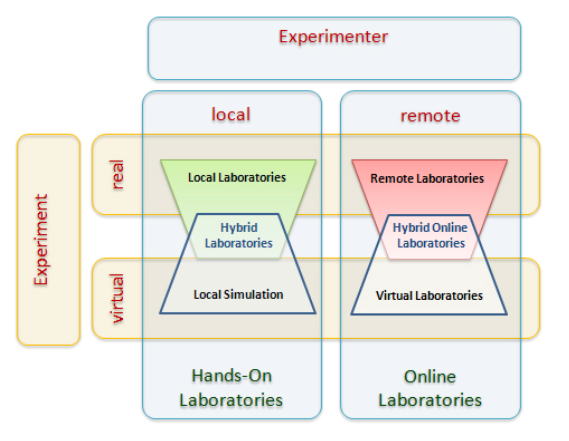
\includegraphics[width=0.65\textwidth]{figures/carac_lab.png}
    \caption{Tipos de laboratórios consoante a localização, segundo Zutin, \textit{et al.} \cite{zutinlab2go}}
    \label{fig:classificaçãozutin}
\end{figure}

Também Heradio, de la Torre e Dormido(2016)\cite{HERADIO20161} classificam os laboratórios de forma idêntica, tal como é representado na Figura \ref{fig:classificaçãoHeratio}:

\begin{figure}[hbtp]
    \centering
    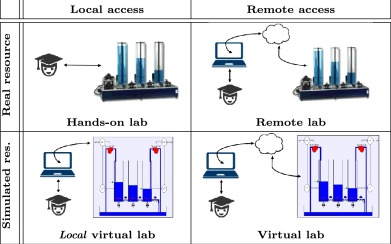
\includegraphics[width=0.65\textwidth]{figures/caracteristica_laboratories.jpg}
    \caption{Tipos de laboratórios consoante a localização, Heradio, de la Torre \& Dormido, (2016) \cite{HERADIO20161}}
    \label{fig:classificaçãoHeratio}
\end{figure}

As representações têm algumas diferenças ao nível da nomenclatura. No entanto, Zutin, \textit{et al.},(2010), \cite{zutinlab2go}, introduzem os conceitos de \textit{Hybrid Laboratories} e \textit{Hybrid Online Laboratories}.
Não é propósito desta dissertação um estudo aprofundado destes conceitos, sendo que o enfoque está no estudo dos laboratórios remotos. Apresenta-se, de qualquer das formas, uma breve explicação dos laboratórios híbridos.

Este tipo de laboratórios é criado através da combinação de laboratórios físicos e/ou laboratórios \textit{online}/remotos \cite{Zapata-Rivera}. Seguem-se alguns exemplos de configurações possíveis:
\begin{itemize}
    \item Acesso a um laboratório real (no local) com acesso local a um \acrfull{lv} - experiência já realizada em contexto de sala de aula: os alunos testam o circuito no \textit{multisim online}, antes de o testarem na placa branca;
    \item Acesso remoto a um laboratório real (no local) e acesso remoto a um \acrshort{lv} - experiência a realizar com os alunos, por exemplo, acedendo ao \acrshort{visir} e simulando o circuito no \textit{multisim online};
    \item Acesso remoto ao laboratório real (no local) e acesso local a um \acrshort{lv} - experiência idêntica à referida no ponto anterior com o \textit{multisim online} a ser substituído pela versão instalada no \acrshort{pc}.
\end{itemize}

Portanto, a forma como são classificados os laboratórios, segundo Heradio, de la Torre \& Dormido,(2016), \cite{HERADIO20161}, representados na Figura \ref{fig:classificaçãoHeratio} - enquadra-se melhor nos conceitos e objectivos abordados neste capítulo:
\begin{itemize}
    \item Acesso local;
          \begin{itemize}
              \item Laboratório real
              \item \acrshort{lv}
          \end{itemize}
    \item Acesso remoto.
          \begin{itemize}
              \item Laboratório remoto
              \item \acrshort{lv}
          \end{itemize}
\end{itemize}

\subsubsection{Uma questão de conceitos}
Antes de mais importa clarificar os conceitos de ``laboratório virtual'' e ``simulador'' (válida para as versões \textit{online} e locais), já que estas duas definições se sobrepõem na maioria dos casos.
Alguma literatura, trabalho de investigação ou informação \textit{online} usam já o termo ``laboratório virtual'' \cite{BRINSON2015218}\cite{virtuallabng}\cite{EMaster2024May}, visto que a montagem nesses sistemas é feita de forma a ter semelhança física com um laboratório real. No entanto, o propósito é o mesmo: o de \textbf{simular}.

\textbf{Uso em sala de aula - REFERIR??}

Nestes dois exemplos demonstrativos\footnote{\textit{Multisim} disponível em \href{https://www.ni.com/en/support/downloads/software-products/download.multisim.html\#452133}{link}} - apresentados na Figura \ref{fig:tinkercad} - o \textit{Tinkercad}\footnote{\url{https://www.tinkerca.com/}} é um \acrshort{lv} e um simulador. O \textit{Multisim}\footnote{\url{https://www.multisim.com/}}, por sua vez, é um simulador, já que a montagem dos circuitos não tem semelhança física com os circuitos montados num laboratório real.

\begin{figure}[hbtp]
    \centering
    \begin{subfigure}[hbtp]{0.48\textwidth}
        \centering
        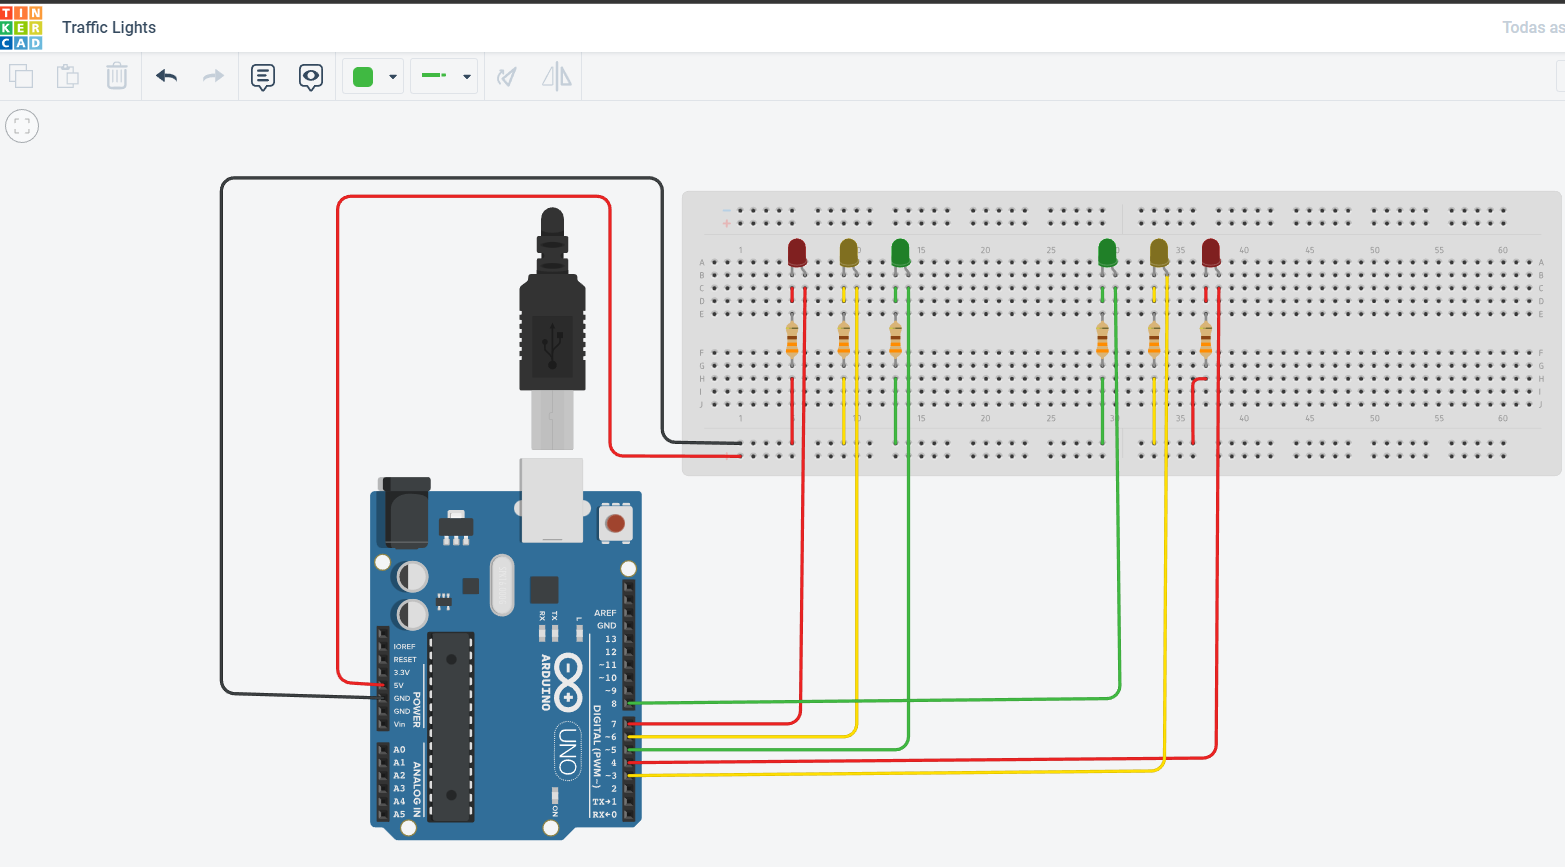
\includegraphics[width=0.9\textwidth]{figures/tinkercad_exemplo.png}
        \caption{\textit{Tinkercad} como \acrshort{lv}}
        \label{fig:tinkercadVL}
    \end{subfigure}
    \begin{subfigure}[hbtp]{0.48\textwidth}
        \includegraphics[width=0.9\textwidth]{figures/Astável-schematic.png}
        \caption{\textit{Multisim} como simulador}
        \label{fig:tinkercadOS}
    \end{subfigure}
    \caption{\acrshort{lv} \textit{vs} simulador}
    \label{fig:tinkercad}
\end{figure}
%…ao contrario do Falstad que simula a partir do esquema.

Na Figura \ref{fig:fritzing}, apresentamos outro exemplo de um \acrshort{lv} recorrendo ao \textit{Fritzing}, que também é um simulador: Tal como foi referido anteriormente, não há um consenso na forma como são denominadas estas ferramentas. Faiña, (2022), \cite{faina}, refere-se ao \textit{Tinkercad} como sendo um simulador, ``Existem vários simuladores destinados a estudantes de eletrónica, como o \textit{TinkerCAD}''. No entanto, no mesmo trabalho de investigação, refere que ``O simulador apresentado neste artigo é implementado no \textit{Fritzing}(\ldots).'' \cite{faina}. Já Knörig, Wettach e Cohen, (2009), no seu artigo ''\textit{Fritzing: a tool for advancing electronic prototyping for designers}`` referem que ``(\ldots) decidiu permitir ao utilizador documentar o seu protótipo de trabalho baseado numa placa de ensaio com uma metáfora visual que imita a situação do utilizador no mundo real.'' \cite{Knorig2009Feb}.

\begin{figure}[hbtp]
    \centering
    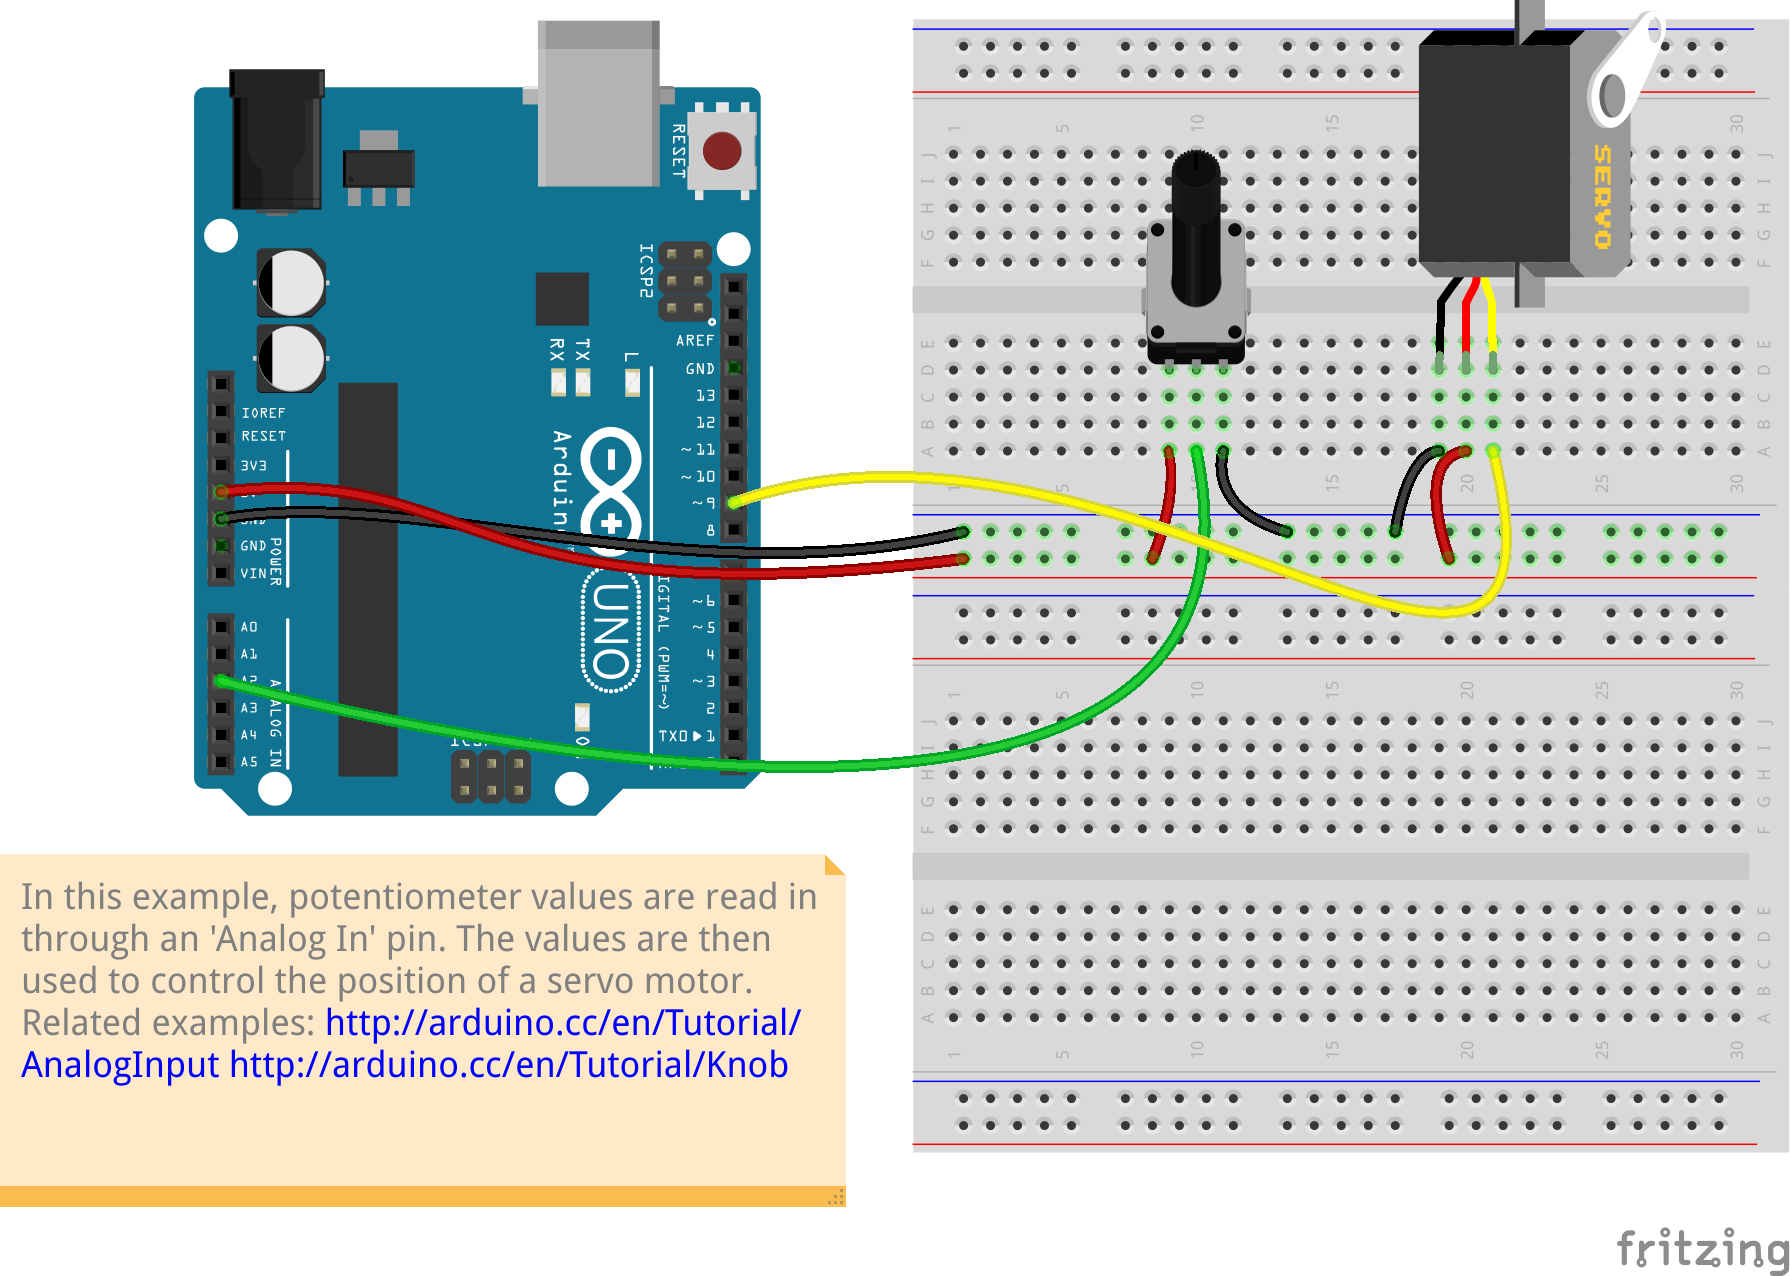
\includegraphics[width=0.9\textwidth]{figures/AnalogInputToServo_bb.png}
    \caption{\textit{Fritzing} (Exemplo)}
    \label{fig:fritzing}
\end{figure}

Além disso, ``(\ldots) um laboratório virtual pode ser definido como um ambiente no qual as experiências são conduzidas ou controladas parcial ou totalmente através de operação, simulação e/ou animação por computador, quer localmente, quer remotamente através da \textit{Internet}.'' \cite{EvaluatingLearningExperiencesVirtualLaboratoryHongKong}. Os laboratórios virtuais oferecem aos alunos um conjunto de oportunidades diferentes, não só como substituto, mas também como complemento dos laboratórios reais.

Assim sendo, e sem prejuízo para os assuntos abordados nesta dissertação, já que não existe uma uniformização dos critérios no que toca às definições e conceitos, é seguro considerar que todos os laboratórios virtuais são simuladores. Heying, Kejie e Jiang, (2010), \cite{multisimVLHeying} e Umenne, Hlalele, (2020), \cite{multisimVLUmenne} consideram nos seus trabalhos de investigação o \textit{Multisim}\cite{multisim} como um \acrshort{lv}. Este conceito é, pois, abrangente o suficiente para abarcar o que se entende por simuladores. Doravante, neste documento, serão considerados e utilizados os termos ``laboratório virtual'' ou ``laboratórios virtuais''.

\subsubsection{Laboratório real}
\textbf{link para não esquecer}
https://digital.dge.mec.pt/laboratorios-de-educacao-digital

Neste tipo de laboratórios, os alunos têm à sua disposição os recursos, o equipamento e os materiais físicos necessários para realizar experiências, analisar dados, desenvolver competências de trabalho em equipa e cultivar o interesse pela ciência, por exemplo. Estas competências são cruciais para muitas carreiras e profissões, especialmente as relacionadas com a ciência, a tecnologia, a engenharia e a matemática - \acrshort{stem}.

Além disso, os laboratórios podem ajudar a melhorar a compreensão dos alunos sobre o processo científico e a importância da investigação científica.

O grande problema dos laboratórios reais é a falta de condições e recursos para os equipar de forma adequada de modo a que possam apoiar, por exemplo, uma turma de trinta alunos. Este não é um problema exclusivamente português, uma vez que, de um modo geral, ``a quantidade de trabalho prático em laboratório no ensino da engenharia tem vindo a ser reduzida pouco a pouco durante as últimas décadas do século passado'' \cite{PaperTit40:online}.

No mesmo artigo \cite{PaperTit40:online} são referidas as principais razões para a diminuição dos laboratórios reais, o que curiosamente reflecte o que se passa atualmente no sistema educativo português:

\begin{itemize}
    \item Número excessivo de alunos por turma \cite{Reduçãod55:online} - embora o número tenha sido reduzido para entre 23-28, para aplicar o ensino laboratorial em contexto de sala de aula, os recursos materiais necessários seriam incomportáveis;
    \item Falta de investimento\cite{Faltadei99:online}, \cite{Odesinve56:online}, \cite{EDUSTATP20:online} - falando por experiência própria, em todas as escolas por onde passamos, a falta de verbas (ou a demora em recebê-las...)'' foi constante; - \textcolor{red}{\textbf{A REVER esta afirmação}}
    \item Custos excessivos dos laboratórios - no contexto português e face a este número de alunos, a montagem e manutenção de um laboratório desta natureza seria demasiado dispendiosa, para além de que os laboratórios não estariam disponíveis durante o tempo que seria desejável;
    \item Falta de professores/Poucos professores - ``Nos próximos sete anos, segundo números do \textit{Conselho Nacional de Educação}, cerca de 20 mil professores do ensino público irão reformar-se. Atualmente, mais de metade dos professores tem 50 anos ou mais.'' \cite{Faltaded39:online}.
\end{itemize}

Sendo assim, que estratégias foram usadas para mitigar estes entraves?

Falando especificamente nos laboratórios do ensino secundário e por experiência própria, uma forma encontrada para equipar os laboratórios passa pela aquisição de \acrfull{microcontroladores} -  nomeadamente, \gls{arduino}s, \gls{ESP32} ou \gls{RaspberryPI}. Todos estes dispositivos - em conjunto com a vasta variedade de sensores disponíveis - já são amplamente utilizados em ambientes educacionais e de pesquisa para a prototipagem rápida, experimentação e aprendizagem prática em engenharia e diversas disciplinas, como eletrónica ou física. Têm como principal vantagem o custo-eficácia. Estes dispositivos e os sensores são relativamente baratos em comparação com equipamentos de laboratório tradicionais, tornando-os acessíveis para escolas e universidades com orçamento limitado. A comunidade de suporte e a documentação é vasta e isso facilita a aprendizagem e a implementação de projetos por estudantes e professores. Com uma enorme gama de sensores e módulos disponíveis no mercado, estes dispositivos podem ser utilizados para criar uma infinidade de experiências e projetos, desde simples medições de temperatura, passando pela robótica até complexos sistemas de automação e controlo.
Em Portugal existem uma série de eventos e competições robóticas, que se destinam a promover o espírito inovador e empreendedor dos alunos, através de métodos activos de ensino, assim como a aquisição de competências transversais. Permitem, ainda, por em prática as aprendizagens realizadas em contexto de sala de aula e em ambiente laboratorial \cite{roboparty}\cite{fnr}\cite{cansat}:
\begin{itemize}
    \item \textit{RoboParty};
    \item Festival Nacional de Robotica;
    \item \textit{Cansat}.
\end{itemize}

Yoder (2015) \cite{yoder}, desenvolveu uma alternativa ao laboratório tradicional recorrendo ao \gls{arduino}: ``(\dots) a plataforma Arduino estimulou o interesse e o envolvimento dos alunos desde o início. Vários alunos começaram a alargar os projectos para além dos requisitos na terceira semana de aulas.''

Graven, \textit{et al},(2018), \cite{graven}, citados por Plaza, \textit{et al.},(2018), \cite{plaza} referem que ``(\ldots) No domínio da educação, o \gls{arduino} é também muito utilizado. Os estudantes de engenharia electrotecnica podem aceder a um laboratório compacto para trabalhar quando e onde quiserem.''. O mesmo autor refere ainda que ``(\ldots) Tal como foi demonstrado por muitas experiências e trabalhos, a robótica combinada com \acrshort{stem} constitui uma forma atractiva de transformar conceitos aborrecidos num processo de aprendizagem divertido.''

Marzoli \textit{et al.},(2021), \cite{Marzoli}, no trabalho de investigação ``Arduino: From Physics to Robotics'', discutem vários pontos e questões, entre os quais se o \gls{arduino} pode melhorar a prática laboratorial no ensino secundário italiano e mudar as atitudes dos alunos em relação às disciplinas \acrshort{stem} e ``Como melhorar as práticas laboratoriais no ensino secundário, tendo em conta os orçamentos e as instalações limitadas disponíveis?''
As conclusões a que chegaram ajudam a revelar a potencialidade do \gls{arduino} em contexto laboratorial: ``A interação profícua entre professores com diferentes formações foi fundamental para a concepção de novas soluções e a exploração de novas aplicações.(\ldots) Assim, o \gls{arduino} pode ser considerado como uma espécie de micro-laboratório (\ldots)''\cite{Marzoli}.

As possibilidades oferecidas por estes dispositivos - nomeadamente, o \gls{arduino} - em contexto de sala de aula e como parte de um laboratório, são imensas, permitindo a realização de uma vasta variedade de projetos inovadores. Esta flexibilidade faz dele uma ferramenta valiosa para a educação e a investigação, facilitando a aprendizagem prática e o desenvolvimento de competências em eletrónica e programação.

\textbf{Uso em sala de aula - REFERIR??}
\begin{figure}[hbtp]
    \centering
    \begin{subfigure}[hbtp]{0.48\textwidth}
        \centering
        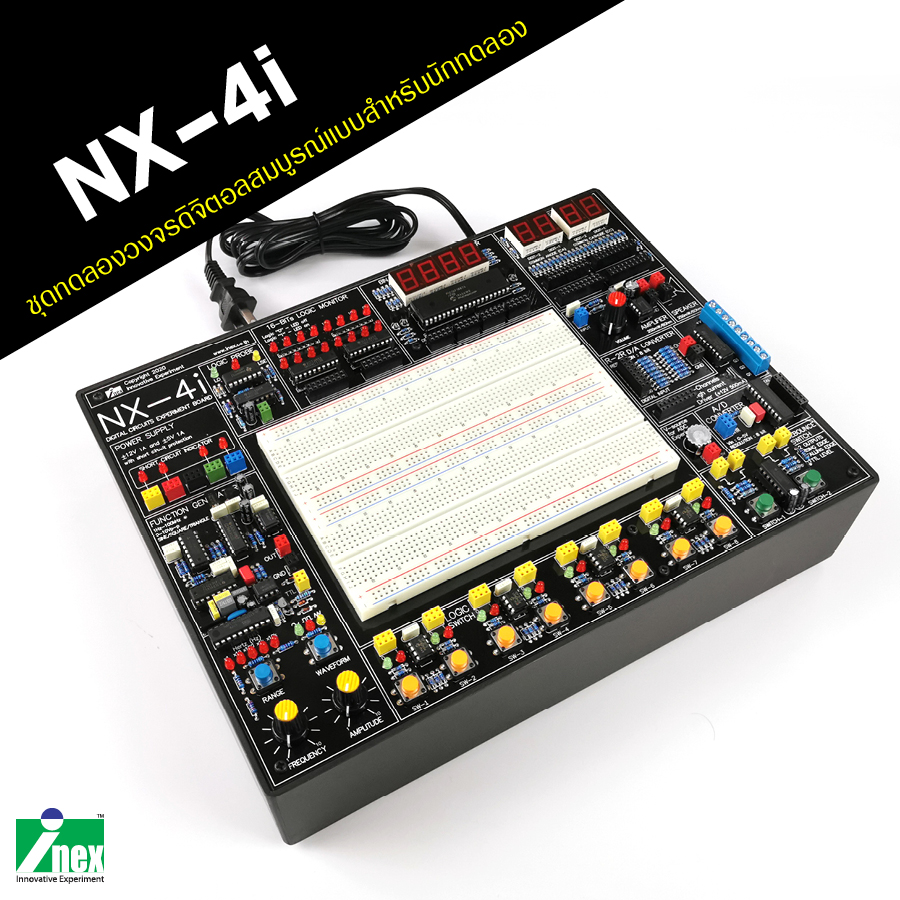
\includegraphics[width=0.9\textwidth]{figures/nx-4i.jpg}
        \caption{\textit{Tinkercad} como \acrshort{lv}}
        \label{fig:nx4i}
    \end{subfigure}
    \begin{subfigure}[hbtp]{0.48\textwidth}
        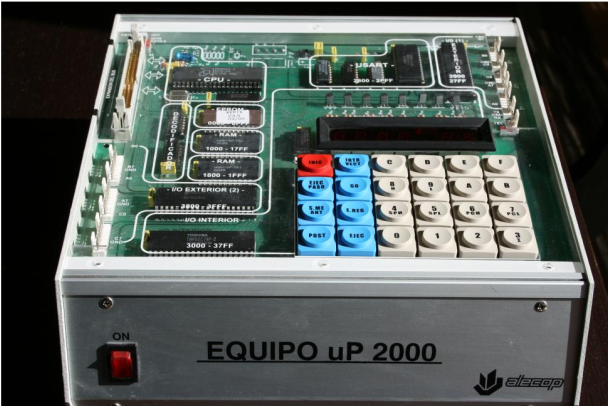
\includegraphics[width=0.9\textwidth]{figures/image-1.png}
        \caption{\textit{Tinkercad} como um simulador \textit{online}}
        \label{fig:up}
    \end{subfigure}
    \caption{Tinkercad}
    \label{fig:lab real}
\end{figure}

\colorbox{yellow}{Colocar fotos?}

\colorbox{yellow}{dar mais algum exemplo do que existe? PocketLAb?}

\colorbox{yellow}{osciloscopio portátilo DSO NANO?}

\colorbox{yellow}{Projecto de uma caixa de sistemas digitais?}

\colorbox{yellow}{A REVER - \textbf{opinião PROF}}


\subsubsection{Laboratório virtual - Acesso local e/ou remoto}
Um \acrshort{lv} é uma poderosa ferramenta que utiliza modelos matemáticos para emular dispositivos reais. Atualmente, os programas de simulação por computador são um padrão de desenvolvimento de produtos aceite pela indústria e são amplamente utilizados no ensino \cite{HERADIO20161} \cite{POTKONJAK2016309}.

No fundo, a diferença entre o acesso remoto e local prende-se com a forma de acesso ao \acrshort{lv}.
Dos programas usados em contexto de sala de aula, só um possui uma versão remota e local: \textit{Multisim}\cite{multisim}. As diferenças situam-se ao nível da \textit{interface} gráfica e, sobretudo, na quantidade de recursos disponível, sendo que na versão local é obviamente muito mais extensa e completa, como se pode ver na Figura \ref{fig:multisimlocal} e Figura \ref{fig:multisimlive}.

O \textit{Tinkercad}\cite{tinkercad} só tem versão \textit{online}, embora se possa instalar um \textit{plug-in} no \acrshort{pc}, que dispensa o uso do navegador. O \textit{Fritzing} \cite{fritzingdown} é acedido localmente, não tendo versão \textit{online}.

\begin{figure}[hbtp]
    \centering
    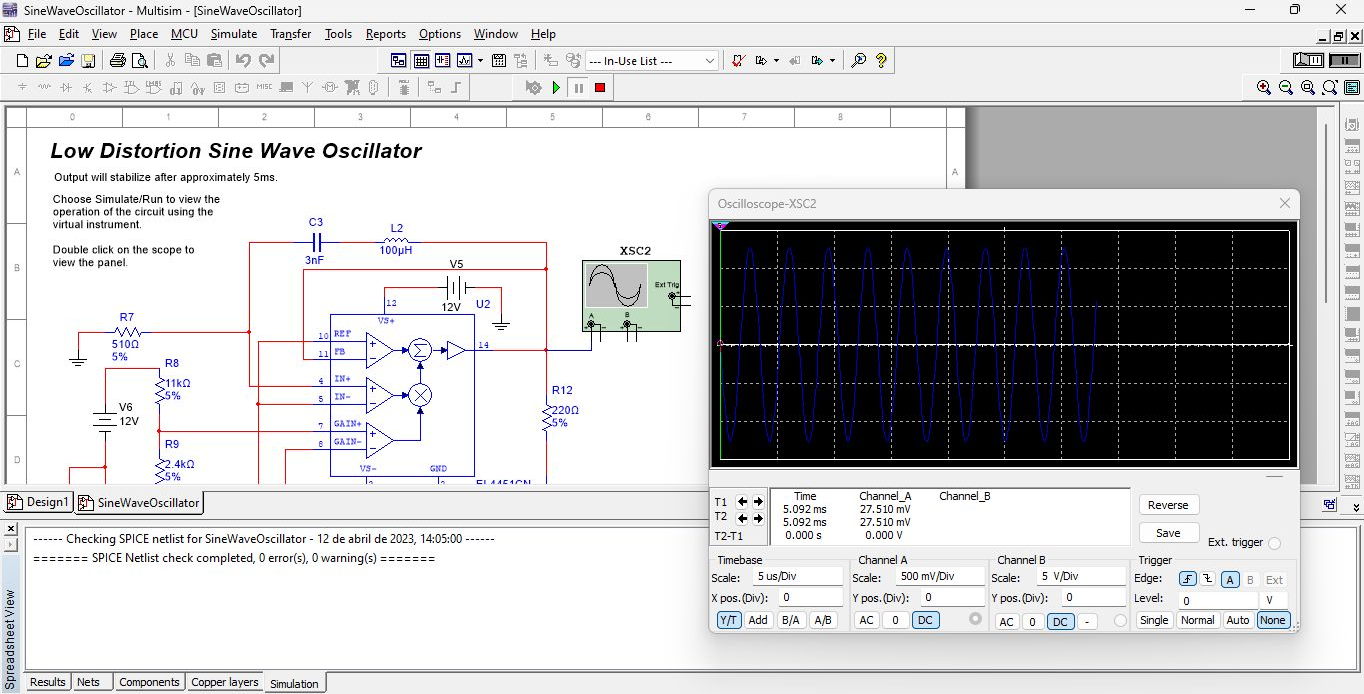
\includegraphics[width=0.9\linewidth]{figures/Multisim_Desktop.png}
    \caption{\textit{Multisim} local}
    \label{fig:multisimlocal}
\end{figure}

\begin{figure}[hbtp]
    \centering
    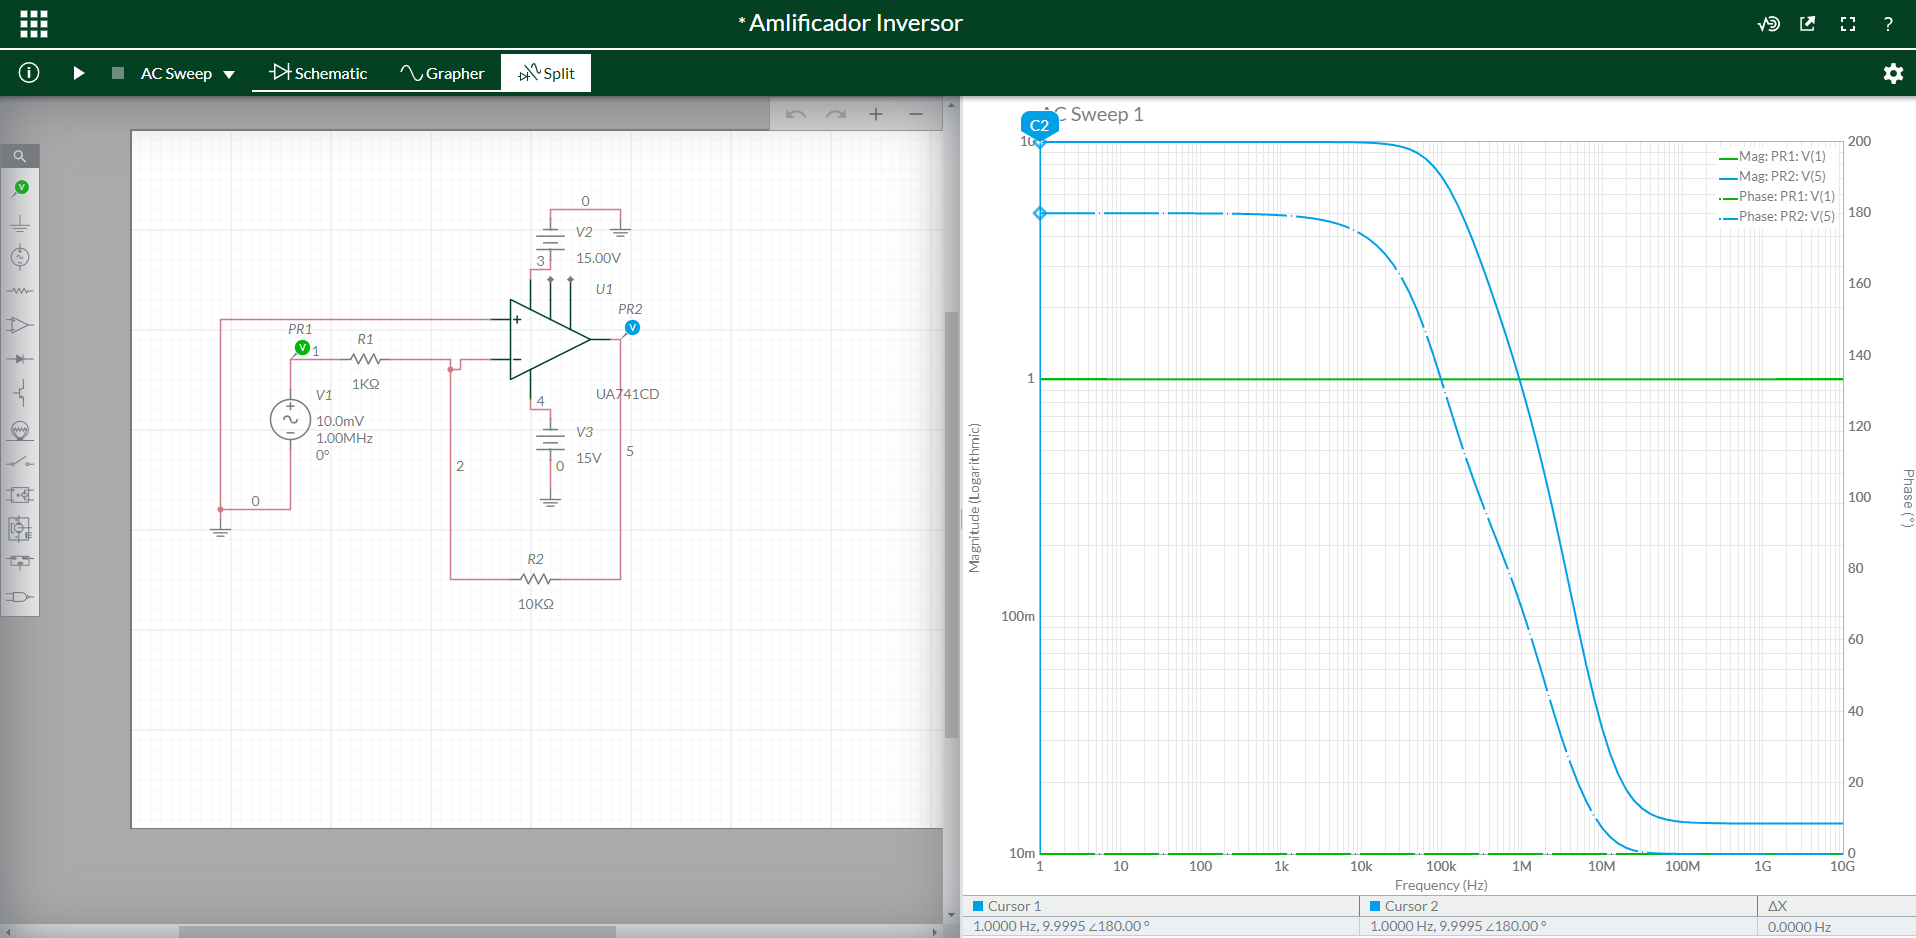
\includegraphics[width=0.9\linewidth]{figures/Multisim_ACsweep.png}
    \caption{\textit{Multisim} remoto}
    \label{fig:multisimlive}
\end{figure}

Estes programas de simulação oferecem aos alunos um conjunto de diferentes oportunidades, não só como substituto, mas também como complemento aos laboratórios reais\cite{WebBrowserSimulators}. Os alunos podem fazer experiências arriscadas sem se porem em perigo. Considerando o nosso caso pessoal, numa turma com 20 ou mais alunos e numa primeira fase, é mais seguro simular um circuito de potência utilizando componentes como \gls{triac}, \gls{diac} ou \gls{scr}. O complemento poderá vir com a montagem real.

Os laboratórios virtuais permitem a verificação e o ensaio de circuitos analógicos e digitais complexos. Têm a capacidade de reproduzir componentes reais com precisão suficiente. As faculdades e universidades de todo o mundo introduzem habitualmente este tipo de \textit{software} de simulação nos cursos de engenharia. Uma vez que todos os circuitos são virtuais, os estudantes podem trabalhar e experimentar uma vasta gama de elementos possíveis sem o perigo de danificar ou destruir o equipamento.

\colorbox{yellow}{esta frase pode ficar mais à frente em jeito de conclusão}
Já foi visto na secção \ref{sec: remotelaboratory} - \textbf{REVER A REFERÊNCIA} que os resultados não são prejudicados pela utilização dos \acrshort{laboratório remoto}s. \textbf{IMPORTANTE - REferências - há um trabalho para apresentar como referência}
No caso de versão do \acrshort{lv} ser remota, as vantagens são semelhantes às de trabalhar com qualquer programa na nuvem:

\begin{itemize}
    \item Não há necessidade de instalar \textit{software} adicional no computador (versão \textit{online});
    \item Desde que a velocidade da \textit{Internet} seja estável, o simulador pode ser acedido em qualquer lugar;
    \item Os circuitos são guardados e armazenados na nuvem;
    \item É ideal para trabalhos colaborativos e partilha de recursos.
\end{itemize}

No entanto, se o \acrshort{lv} for apresentado uma versão de acesso local, ou seja, que é instalada no \acrshort{pc}, é óbvio que estas vantagens não se aplicam.

Mas as vantagens dos \acrshort{lv}s vão muito para além das descritas em anteriormente \cite{scheckler}\cite{lynch}\cite{BlogeMas95}\cite{vabtegensVL}.
Oferecem um ambiente seguro para a realização de experiências complexas e (potencialmente) perigosas, reduzindo os riscos para os estudantes e professores. Os estudantes podem podem progredir ao seu próprio ritmo e repetir as experiências as vezes que forem necessárias, estando os laboratórios acessíveis a qualquer altura e em qualquer lugar. Os laboratórios virtuais são, por inerência, mais baratos, de fácil instalação e manutenção e - a juntar a estes factos vantajosos - há ainda informação de ajuda e tutoriais \textit{online}.

Mas os laboratórios virtuais também têm as suas desvantagens. A principal pretende-se com o desfasamento da realidade. Pegando no exemplo anterior - a simulação de circuitos de potência - o facto de nada de mau poder acontecer pode levar a uma atitude de desresponsabilização ou falta de cuidado, já que o estudante pode ser levado a pensar que nada de grave poderá acontecer \cite{POTKONJAK2016309}. Há sempre constrangimentos no que diz respeito à evolução tecnológica dos sistemas que suportam o \acrshort{lv}, assim como à disponibilidade de uma ligação à \textit{Internet} adequada ao seu uso. Se não for usado em contexto de sala de aula, o \acrshort{lv} reduz a interação direta entre os alunos e entre estes e os professores, uma vez que a comunicação é sobretudo feita \textit{online}. Além do mais, exige do aluno mais iniciativa e autonomia. Há ainda a referir algumas vantagens que se podem tornar desvantagens. O facto de o aluno poder testar e simular vezes sem conta, acabará por lhe retirar sensibilidade quando utilizar os laboratórios e componentes reais; a imensa quantidade de informação disponível \textit{online} terá que ser ``filtrada'' pelo aluno\cite{POTKONJAK2016309}\cite{vabtegensVL}\cite{Gherasim}\cite{Ghergulescu2019Feb}.

Um dos principais simuladores disponíveis gratuitamente, embora com limitações de funcionalidades, usado numa base regular em contexto de sala de aula, é o \textit{Multisim}\cite{multisim}. Em tempos de confinamento, este \acrshort{lv} foi um ``salva-vidas''. Existe também uma versão \textit{premium} que oferece acesso a uma gama mais completa de recursos \textit{online} e uma versão que pode ser instalada no \acrshort{pc}. (O funcionamento destas duas versões é em tudo idêntico, portanto, quando nos referirmos ao \textit{Multisim}\cite{multisim}, entende-se as duas versões, sem perda de generalidade. Nos casos em que houver necessidade de distinção, esse facto será devidamente referenciado).
Este \textit{software} integra a simulação virtual \acrfull{spice} padrão da indústria com um ambiente esquemático interativo para visualizar e analisar instantaneamente o comportamento de circuitos electrónicos. É uma ferramenta poderosa que utiliza modelos matemáticos para simular componentes reais, dispositivos ou circuitos com uma precisão muito boa, através de um navegador \textit{web}. Fornece uma plataforma para ``colmatar'' a lacuna entre a teoria dos manuais e os circuitos reais e também proporciona aos estudantes uma boa plataforma para experiências abrangentes e inovadoras\cite{multisim}.

Além disso, dispondo de poderosas funcionalidades de aprendizagem e integração de \textit{hardware} de laboratório, o \textit{Multisim} ensina aos alunos conceitos fundamentais de eletrónica analógica, digital e de potência presentes em todo o currículo de engenharia e ciências \cite{ImportantSimSoftware}.

Citando Heying, Kejie e Li, (2010), ``(\ldots) podemos concluir que a criação de uma plataforma de simulação virtual através do \textit{Multisim} num computador permite construir facilmente todo o tipo de circuitos. (\ldots) Seguem-se os comentários de alguns alunos:''
\begin{itemize}
    \item ``O ensino experimental utilizando o \textit{Multisim} é uma boa abordagem para me ajudar a compreender as matérias;''
    \item ``Gostei de trabalhar na plataforma de simulação virtual \textit{Multisim}'';
    \item ``A simulação \textit{Multisim} ajudou-me a compreender melhor as experiências.''
\end{itemize}

Os mesmos autores concluem que: ``O laboratório virtual [\textit{Multisim}] desempenha um papel muito importante na atualização do método de ensino experimental, na melhoria da qualidade do ensino dos cursos em circuito e na otimização do efeito do ensino.''\cite{heying}

Outro laboratório bastante usado em contexto de sala de aula foi criado e desenvolvido por \textit{Paul Falstad}, em 1985 e está disponível em \href{www.falstad.com}{Falstad} \cite{falstad}. Este \acrshort{lv} é livre e de código aberto \cite{falstadlicenca}. Funciona num navegador \textit{web} como uma \textit{applet JAVA}. É também importante por ser de fácil interacção e pela simplicidade na representação de circuitos eléctricos, aspectos muito importantes para os recursos multimédia nas áreas da electrónica e da electricidade\footnote{Para sermos mais rigorosos, este \acrshort{lv} não se cinge somente aos circuitos electrónicos, ligando-se também a outros ramos da ciência como a termodinâmica, a mecânica quântica, o processamento de sinal, etc. \cite{falstadcompleto}}.

Além disso, o simulador \textit{Falstad} tem sido desenvolvido como uma aplicação de \textit{Internet} há muitos anos, segundo da Silva \textit{et al.}, (2011), \cite{RemoteTeachingElectricalCircuits}, citados por \textit{Falstad},(2024), \cite{falstad}.

O principal problema é que, devido à falta de parametrização avançada e de um modelo matemático, este \acrshort{lv} não se destina a engenharia profissional ou real. No entanto, para fins didácticos, é muito eficaz. Por exemplo, é de referir que:
\begin{itemize}
    \item Os pontos amarelos animados representam correntes e os seus movimentos demonstram um fluxo de cargas eléctricas em ''tempo real``;
    \item De acordo com a direção do fluxo da corrente, a cor do fio é representada por verde ou vermelho, tendo em conta a direcção do fluxo da corrente;
    \item Os componentes mostram diferentes tensões no circuito;
    \item As formas de onda também são representadas;
    \item Podem ser representados e controlados diferentes tipos de interruptores, por exemplo, para fazer variar frequência e/ou tensão, Figura \ref{fig:falstad}, o que permite o utilizador observar os processos transitórios;
    \item A velocidade da simulação e a corrente também podem ser controladas.
\end{itemize}

\begin{figure}[hbtp]
    \centering
    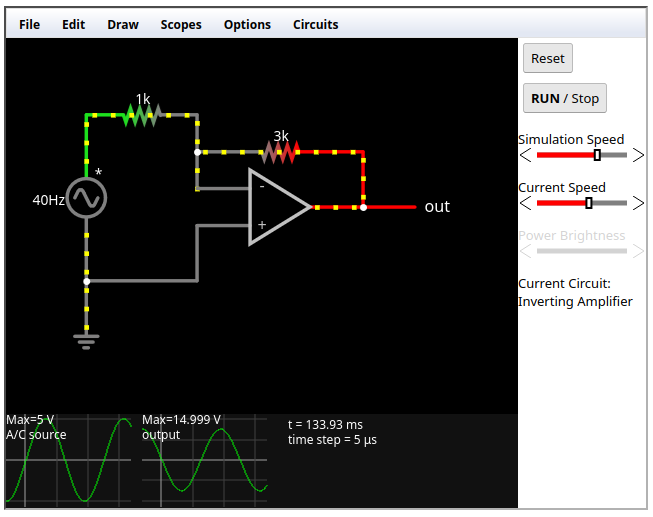
\includegraphics[width=0.75\textwidth]{figures/falstad.png}
    \caption{\textit{Falstad} - amplificador inversor\cite{falstad}}
    \label{fig:falstad}
\end{figure}

A variedade de laboratórios virtuais no contexto da electrónica é muita, pelo que só referimos os mais usados em contexto de sala de aula. No entanto, outras soluções seriam de considerar, tais como:
\begin{itemize}
    \item \textit{Tinkercad} - é uma aplicação \textit{online} gratuita para projetos 3D, de eletrónica e de programação;
    \item \textit{Fritzing} - a \textit{interface} é muito semelhante à do \textit{TinkerCad}, com a excepção de não poder realizar simulações, no entanto, fornece uma variedade muito maior de componentes do que o \textit{TinkerCad};
    \item \textit{Wokwi}\cite{wokwi} - \acrshort{lv} que usa as mais variadas placas que simulam o \gls{arduino}, \gls{ESP32}, \textit{STM32}, \textit{RaspberryPi Pico} e uma grande variedade de sensores\cite{wokwi}.
\end{itemize}

\colorbox{yellow}{\textbf{FALTA AQUI UMC CONCLUZÃOZINHA}}

\subsubsection{Laboratório remoto}
\label{sec: remotelaboratory}
Alguns dos problemas dos laboratórios reais já foram abordados ao longo destes dois capítulos. As vantagens são bastante evidentes e prendem-se, sobretudo, com a possibilidade de os alunos trabalharem utilizando recursos físicos. No entanto, no ensino secundário, nem sempre é possível ter acesso a esses recursos, quer por dificuldades em obter os fundos necessários para manter um laboratório, quer porque é simplesmente incomportável montar um laboratório onde vinte ou vinte e quatro alunos possam realizar experiências ao mesmo tempo. No ensino superior, em que, pelo menos teoricamente, os alunos são mais autónomos do que no ensino secundário, o principal problema é a disponibilidade de laboratórios fora das aulas normais.

Numa época em que a tecnologia é cada vez mais encarada como um facilitador no processo de ensino/aprendizagem, a utilização de laboratórios remotos é cada vez mais comum e generalizada. Além disso, os laboratórios remotos apresentam algumas vantagens em relação aos laboratórios reais e mesmo aos simuladores \cite{RemoteLabsImpactVISIR}, tais como: flexibilidade, acessibilidade, disponibilidade e segurança.

\textcolor{red}{\textbf{ATENÇÃO AOS ACRÓNIMOS DESTE PARÁGRAFO}}Estes tipos de laboratórios - que incluem, por exemplo, o \acrshort{visir}, o \textit{LabsLand}\footnote{\url{https://labsland.com/en}} ou o \textit{WebLab-Deusto}\footnote{\url{https://weblab.deusto.es/website/}} - permitem que professores/investigadores e alunos acedam a equipamentos e/ou computadores através da Internet para realizar experiências e tarefas laboratoriais sem estarem no espaço físico dos laboratórios \cite{ExperiencesRemoteLab}.

Num \acrshort{laboratório remoto}, a interação tem lugar à distância com a ajuda da infraestrutura remota. Esta é uma nova camada que se situa entre o utilizador e o equipamento do laboratório. É responsável pela transmissão das acções do utilizador e pela receção da informação sensorial do equipamento.
Várias investigações mostram que os estudantes podem efetivamente aprender com a utilização de laboratórios remotos e também de laboratórios virtuais, obviamente se estiverem empenhados no que estão a estudar \cite{RemoteLabsImpactVISIR}.

De acordo com Viegas \textit{et al.}, (2018)\cite{ImpactRemoteLabTeachingPractices}, citando Brinson, (2015)\cite{BRINSON2015218} e Corter \textit{et al.}, (2011)\cite{CORTER20112054}, os resultados obtidos com simuladores e laboratórios remotos podem ser considerados semelhantes ou mesmo superiores aos dos laboratórios práticos reais. No entanto, uma abordagem à aprendizagem laboratorial que utilize uma combinação de laboratórios práticos, simulações e procedimentos de laboratórios remotos parece ser a forma mais eficaz de aprendizagem, tirando partido dos benefícios dos três \cite{BRINSON2015218}.

Esta mesma conclusão foi obtida por de Mel e Samaranayaka, (2017), no estudo intitulado ``Extending the boundaries of remote laboratory by providing hands on experience''. Citando os autores: ``(\ldots) os estudantes estão disponíveis a usar o \acrshort{laboratório remoto} juntamente com o real (\ldots)'', mas ``(\ldots) não aconselham a total substituição (\ldots)''. O estudo conclui, ainda, que não há grande diferença entre o laboratório real e remoto, sendo que os conhecimentos adquiridos são (praticamente) os mesmos\cite{deMel}.

Podem ser considerados outros estudos que, por exemplo, comparem laboratórios reais (práticos) e simulados, laboratórios reais e virtuais. De facto, Corter \textit{et al.}, (2007) concluem que ``(\ldots) os laboratórios remotos e simulados podem ser pelo menos tão eficazes como os laboratórios práticos tradicionais no ensino de conceitos específicos da disciplina''\cite{StudyRemoteHandsonSimulatedLabs}. Outro estudo feito por Kocijancic e O'Sullivan, (2004) conclui que ``(\ldots) não se trata de saber se é melhor utilizar experiências reais ou laboratórios virtuais no ensino das ciências, uma vez que ambas as abordagens, utilizadas de forma complementar, podem contribuir para uma aprendizagem ativa mais eficaz.'' \cite{RealorVirtualDilema}. Tsihouridis \textit{et al.}, (2019), concluem também que ``não há um vencedor final nesta controvérsia intemporal entre os dois ambientes de laboratório experimental, de acordo com a nossa investigação.'' \cite{controversy}.

Assim, através de estudos efectuados, será seguro afirmar que os laboratórios remotos são a melhor alternativa aos tradicionais em termos de baixo custo e ubiquidade, e algumas universidades já começaram a recorrer a laboratórios remotos nas suas sessões práticas\cite{VISIREngineeringPractices}. \textbf{\textcolor{red}{REVER esta frase em jeito de conclusão!}}

De facto, de acordo com Nafalski \textit{et al.}, (2010)\cite{ExperiencesRemoteLaboratories}, citando Auer e Gravier, (2009)\cite{ThemMnyfacesRemotLab} as razões para o crescimento dos laboratórios remotos em engenharia e ciência prendem-se com:

\begin{itemize}
    \item A crescente complexidade das tarefas de engenharia;
    \item O equipamento cada vez mais especializado e dispendioso, as ferramentas de software e os simuladores necessários;
    \item A necessidade de utilizar equipamentos e ferramentas de \textit{software}/simuladores dispendiosos em projectos com prazos curtos (como os apresentados em \cite{ExperiencesRemoteLab});
    \item A aplicação de equipamentos de alta tecnologia necessários em pequenas e médias empresas;
    \item A necessidade de pessoal altamente qualificado para controlar os novos equipamentos;
    \item As exigências da globalização e da divisão do trabalho.
\end{itemize}

No entanto, se se pretende, segundo Fan, Evangelista e Indumathi, (2021), \cite{EvaluationRemoteVirtualE-Learning}, citando Tawfik \textit{et al.}(2016)\cite{RemoteLabsImpactVISIR}, Chen \textit{et al.}, (2010)\cite{DevelopingVirtualAndRemoteUndergraduate} e Simão \textit{et al.}, (2014), \cite{RemoteLabsDevelopingCountries}, incorporar os laboratórios remotos com \gls{industria40}, já discutidas no Capítulo \ref{Capítulo1}, tem vantagens óbvias:
\begin{itemize}
    \item Os estudantes podem fazer os exercícios da disciplina ao seu próprio ritmo e de acordo com o seu nível de interesse;
    \item A quantidade de tempo (muitas vezes horas extraordinárias) que os professores têm de despender na preparação e ensino dos laboratórios pode ser reduzida;
    \item Podem ser efectuadas várias experiências utilizando a mesma configuração;
    \item Os laboratórios remotos permitem o acesso de um maior número de utilizadores, o que significa que a sua instalação acaba por ser mais barata do que a dos laboratórios físicos;
    \item Os laboratórios remotos estão acessíveis 24 horas por dia, 7 dias por semana;
    \item Os laboratórios remotos podem ajudar a reforçar o trabalho autónomo dos alunos;
    \item Os laboratórios remotos são mais seguros, tanto para o utilizador como para o equipamento ou software, uma vez que estão fisicamente separados e são orientados para a tecnologia.
\end{itemize}

Embora os laboratórios remotos ofereçam muitas vantagens, como as descritas em cima, é importante estar ciente das suas desvantagens (muitas delas comuns com as descritas para os laboratórios virtuais). A falta de interacção física directa, a dependência da ligação com a \textit{Internet}, os desafios técnicos e de manutenção, a experiência de aprendizagem menos imersiva e a limitação da interação com colegas e professores são pontos críticos que devem ser considerados ao implementar esses laboratórios. No entanto, a principal desvantagem dos laboratórios remotos, prende-se com a complexidade da sua implementação. Como os \acrshort{laboratório remoto}s seguem uma arquitectura cliente-servidor, além do servidor é ainda necessário ter em conta a questão do \textit{hardware} e a sua integração com o \textit{software} que pode, ou não, ser proprietário. Há ainda a questão essencial da forma como os utilizadores acedem ao laboratório. Isto levanta problemas de largura de banda, que restringe o número de utilizadores que podem aceder simultaneamente ao \acrshort{laboratório remoto} \cite{HERADIO20161}.

Sendo assim, os laboratórios remotos não são simplesmente uma versão reduzida de um laboratório real (prático), mas uma abordagem diferente com pontos fortes e fracos alternativos, oferecendo novas oportunidades que não são proporcionadas pelas abordagens tradicionais. No final, se forem combinados e complementados com laboratórios reais e simulações, é possível tirar partido das vantagens que estes três tipos de laboratórios proporcionam.

%Quanto à implementação dum laboratório remoto, a quantidade de soluções que existem é vasta. 
Existem muitos tipos de laboratórios nos mais variados campos da ciência (Física, Electrónica, Robótica ou Química) e com os mais variados tipos de arquitectura de \textit{hardware} e \textit{software}. Apesar de não estar no objectivos desta dissertação um estudo aprofundado desta matéria, ficam alguns exemplos que esclarecem e atestam o quão vasto, complexo e variado é este assunto.
\colorbox{yellow}{vale a pena fotos? PROF?}

Dentro dos laboratórios remotos que existem e actualmente estão activos, destacam - se os seguintes:
\begin{itemize}
    \item \acrshort{visir} - é um \acrshort{laboratório remoto} que interliga vários componentes reais, que podem ser ligados para realizar diferentes tarefas e para construir circuitos específicos concebidos pelo utilizador final, como se pode ver na Figura \ref{fig:visirISEP}; permite a estudantes e professores fazerem medições reais em circuitos reais, algo que não é possível em simulações; será discutido com mais pormenor mais adiante;
    \item A Universidade de \textit{Deusto}, em Bilbao tem disponível uma conjunto de \acrshort{laboratório remoto}s, que inclui o \acrshort{visir}, o comando de um robô através de um \gls{arduino} ou a programação de uma \acrfull{fpga};
          %\textit{WebLab-Deusto} - O \textit{WebLab-Deusto} é uma iniciativa da Universidade de Deusto com o objetivo de aumentar a aprendizagem experimental através da utilização e desenvolvimento de laboratórios remotos
    \item \textit{iSES}\footnote{\url{https://www.ises.info/index.php/en/systemises/sdkisesstudio}} - tem várias experiências remotas que abrangem diversas áreas da ciências, como Física, Electrónica, Radioactividade, Electromagnetismo, etc.
    \item \textit{OpenSTEM}\footnote{\url{https://learn5.open.ac.uk/}} - estes laboratórios têm uma colecção de experiências abrangendo áreas científicas que vão desde a saúde, engenharia ou observatórios;
    \item \textit{Remote-LAB GymKT}\footnote{\url{http://remote-lab.fyzika.net/}} - Várias experiências que vão desde o controlo de um braço robótico através de um \gls{arduino} até experiências no campo da física e da electrónica;
\end{itemize}

No entanto, a implementação dos laboratórios remotos assenta sobre as mais variadas, e complexas, soluções.
\begin{figure}[hbtp]
    \centering
    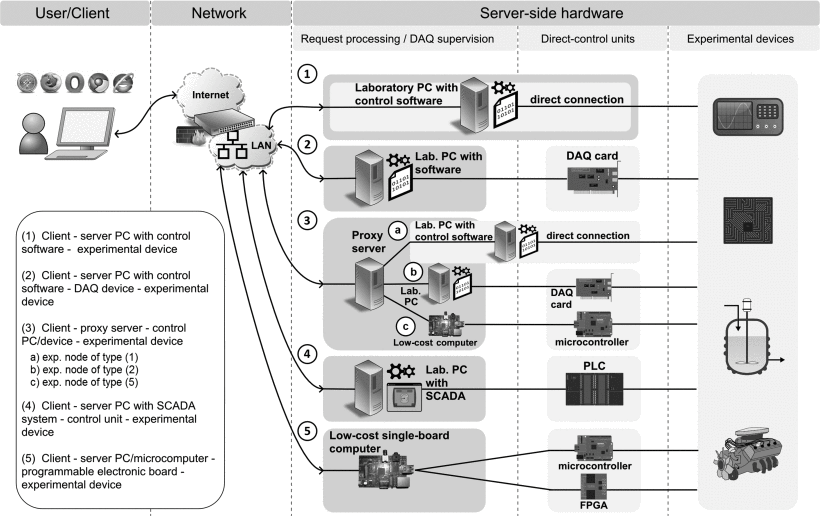
\includegraphics[width=0.75\textwidth]{figures/kaluz.png}
    \caption{Diferentes tipos de arquitectura (resumo)}
    \label{fig:diferentestiposarq}
\end{figure}

Segundo Kalúz \textit{et al.}, (2015), Figura \ref{fig:diferentestiposarq}, os tipos mais frequentes de arquitecturas são\cite{Kaluz}:
\begin{itemize}
    \item Cliente-servidor com \textit{software} de controlo - dispositivo experimental: este tipo de arquitetura muito comum utiliza uma ligação direta entre o \acrshort{pc}(servidor) e o dispositivo controlado, por exemplo, através de uma porta série ou \acrfull{usb};
    \item Cliente-servidor com \textit{software} de controlo - dispositivo de aquisição de dados (\acrfull{daq});
    \item Configuração experimental remota com funcionalidade muito semelhante à anterior; a única diferença é que o dispositivo de aquisição de dados (normalmente uma placa \acrshort{daq}) é uma parte separada da arquitetura;
    \item Nós cliente-servidor-\textit{proxy}-laboratório (\acrshort{pc} + unidade de controlo)-dispositivos experimentais: este tipo, também conhecido como arquitetura ramificada, oferece uma maior capacidade de possíveis ligações experimentais do que qualquer outra arquitetura;
    \item Cliente-servidor com sistema de controlo de supervisão e aquisição de dados (\acrfull{scada}) - unidade de controlo - dispositivo experimental: a combinação do sistema \acrshort{scada} com uma unidade de controlo (\acrfull{plc} ou outro controlador de \textit{hardware}) é uma das abordagens industriais mais frequentemente utilizadas;
    \item Cliente - servidor/microcomputador - placa eletrónica programável - dispositivo experimental: as abordagens muito populares nos últimos anos, também frequentemente designadas na literatura como de baixo custo, baseiam-se em placas programáveis como as \acrshort{fpga}, microcontroladores \gls{arduino} e alternativas baratas aos computadores normais (por exemplo, computadores de placa única baseados na arquitetura \acrfull{arm}, como \gls{RaspberryPI}, entre outros);
    \item \textit{\acrfull{mhsa}}: é composto por uma arquitetura de \textit{hardware}, baseada em dispositivos industriais, que permite ao programador ligar vários tipos de experiências à sua configuração física, limitada apenas pelas capacidades de ligação dos nós experimentais e por um \textit{software} baseado na \textit{web} do lado do cliente, que proporciona uma grande versatilidade tanto para a implementação final como para a utilização; desde o início, o \acrshort{mhsa} foi desenvolvido como uma arquitetura para a implementação de laboratórios de sistemas de controlo, sem ter em conta a utilização de dispositivos específicos, reduzindo o \textit{back-end} a um conjunto de sinais.
\end{itemize}

Fabregas \textit{et al.}, (2011), utilizam o \textit{Simulink}, do lado do servidor, e o \acrfull{ejs}, do lado do cliente, para realizar a implementação do \acrshort{laboratório remoto}\cite{FABREGAS20111686}, Figura \ref{fig:ejs}.
\begin{figure}[hbtp]
    \centering
    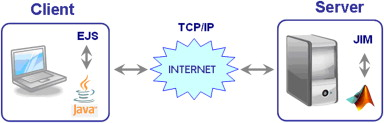
\includegraphics[width=0.75\textwidth]{figures/sej.jpg}
    \caption{Implementação cliente-servidor \acrshort{matlab}-\acrshort{ejs}}
    \label{fig:ejs}
\end{figure}
Ainda no mesmo artigo - Lazar e Carari, (2008) - desenvolveram um \acrshort{laboratório remoto} baseado no \textit{software} \textit{LOOKOUT SCADA} da \acrfull{ni}, \cite{lazar} citado por \cite{FABREGAS20111686}.
Por sua vez, Dormido \textit{et al.}, (2008), desenvolveram um \acrshort{laboratório remoto}, em que o \acrfull{labview} estava implementado no servidor, \cite{dormido} citado por \cite{FABREGAS20111686}. Em ambas implementações foi utilizada uma arquitectura cliente-servidor.

A \acrfull{diesel} é outro tipo de arquitectura que é aplicada na implementação de laboratórios remotos. A abordagem cliente-servidor do \acrshort{diesel} utiliza uma arquitetura de \textit{software} distribuída, desenvolvida com a tecnologia \textit{Microsoft .NET}. É constituída por uma aplicação cliente, um determinado número de estações de trabalho experimentais que alojam aplicações servidoras individuais, um servidor \textit{Web} que aloja uma base de dados, um serviço \textit{Web} e um sistema de reservas baseado na \textit{Web} \cite{diesel}, como se pode ver na Figura \ref{fig:resumoarquitectura}.
\begin{figure}[hbtp]
    \centering
    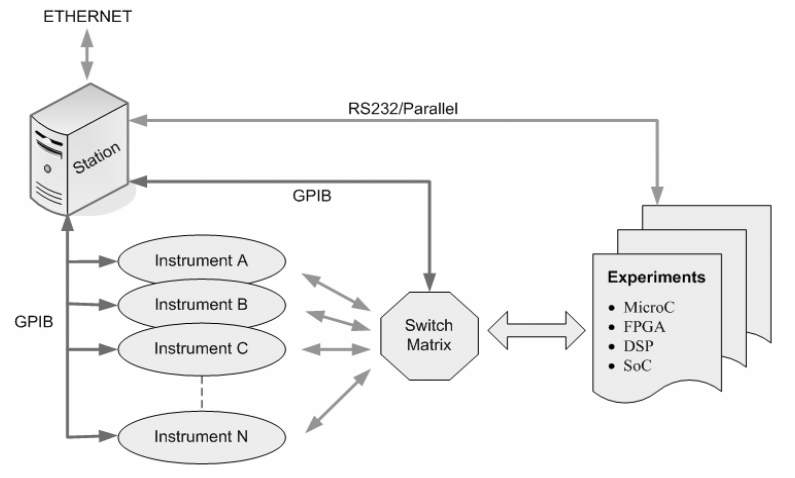
\includegraphics[width=0.75\textwidth]{figures/diesel.png}
    \caption{Arquitectura \acrshort{diesel} (genérica)\cite{diesel}}
    \label{fig:resumoarquitectura}
\end{figure}

Jacko \textit{et al.}, (2022) - no seu artigo ``Remote IoT Education Laboratory for Microcontrollers Based on the STM32 Chips'' - descrevem a implementação de um \acrshort{laboratório remoto} que utiliza o \textit{Microsoft Visual Studio} 2019 do lado do servidor \cite{jacko}.

Candelas \textit{et al.}, (2003), implementaram um \acrshort{laboratório remoto} dedicado ao ensino da robótica em que a ``ponte'' entre a experiência e o utilizador é feita atráves de \textit{Java Applet}.

No entanto, a implementação dos \acrshort{laboratório remoto}s vai muito para além dos conceitos abordados anteriormente, a \textbf{Interoperabilidade} torna possível a integração de diferentes \acrshort{laboratório remoto}s mas levanta outro tipo de problemas, como sendo a gestão dos \acrshort{laboratório remoto}s e funcionalidades, autenticação, autorização ou gestão de utilizadores. Este facto abriu espaços à criação de serviços que pudessem gerir estas funcionalidades, comummente designados por \acrfull{rlms}. Trata-se de \textit{software} de gestão que pode suportar vários laboratórios remotos (por exemplo, um laboratório de robótica e um laboratório de eletrónica ao mesmo tempo) e fornece autenticação, autorização, gestão de utilizadores, monitorização de utilizadores e agendamento, bem como \acrfull{api}s para desenvolvimento de novas funcionalidades e laboratórios \cite{Vocabulariog4l}.

A \acrfull{ilab}\footnote{\url{https://icampus.mit.edu/projects/ilabs/\#architecture}}, Figura \ref{fig:arquitecturaisa}, é uma arquitetura de software, desenvolvida pelo \acrfull{mit}, que oferece aos criadores e utilizadores dos \acrshort{laboratório remoto}s uma estrutura comum para utilizar, partilhar e disponibilizar mecanismos para a partilha de \acrshort{laboratório remoto}s numa arquitetura distribuída baseada em serviços \textit{Web}, gerindo o agendamento e a manutenção de sessões de laboratório durante a execução de uma experiência\cite{zutin}. Os utilizadores acedem a estes \acrshort{laboratório remoto}s através de um início de sessão único e de uma \textit{interface} administrativa normalizada simples. O projeto \acrshort{ilab} demonstrou que a utilização de laboratórios pode ser alargada a milhares de estudantes dispersos globalmente\cite{harward}\cite{arquitecturaisa}. Zutin, Auer e Gustavsson, (2011), apresentaram uma solução para integrar o \acrshort{visir} no \acrshort{ilab}\cite{zutinvisir}.

\begin{figure}[hbtp]
    \centering
    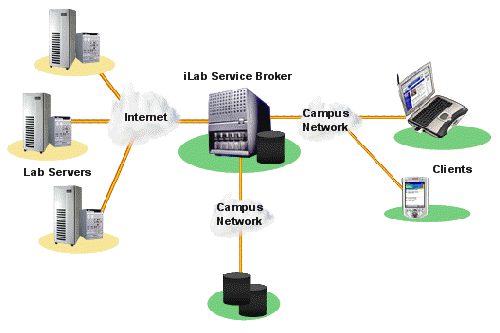
\includegraphics[width=0.8\textwidth]{figures/isa_architecture.png}
    \caption{Arquitectura \acrshort{ilab}\cite{arquitecturaisa}}
    \label{fig:arquitecturaisa}
\end{figure}

O \textit{WebLab-Deusto} é uma iniciativa desenvolvida pela Universidade de Deusto\footnote{\url{https://www.deusto.es/es/inicio}}, Bilbao, e consiste num sistema de gestão de \acrshort{laboratório remoto} de código de fonte aberto (\textit{BSD 2-clause license}). A arquitectura do \textit{WebLab-Deusto} é definida localmente e baseia-se na arquitetura distribuída cliente-servidor \textbf{MODULAR? REVER}, como podemos ver na Figura \ref{fig:arquitecturawld}.

\begin{figure}[hbtp]
    \centering
    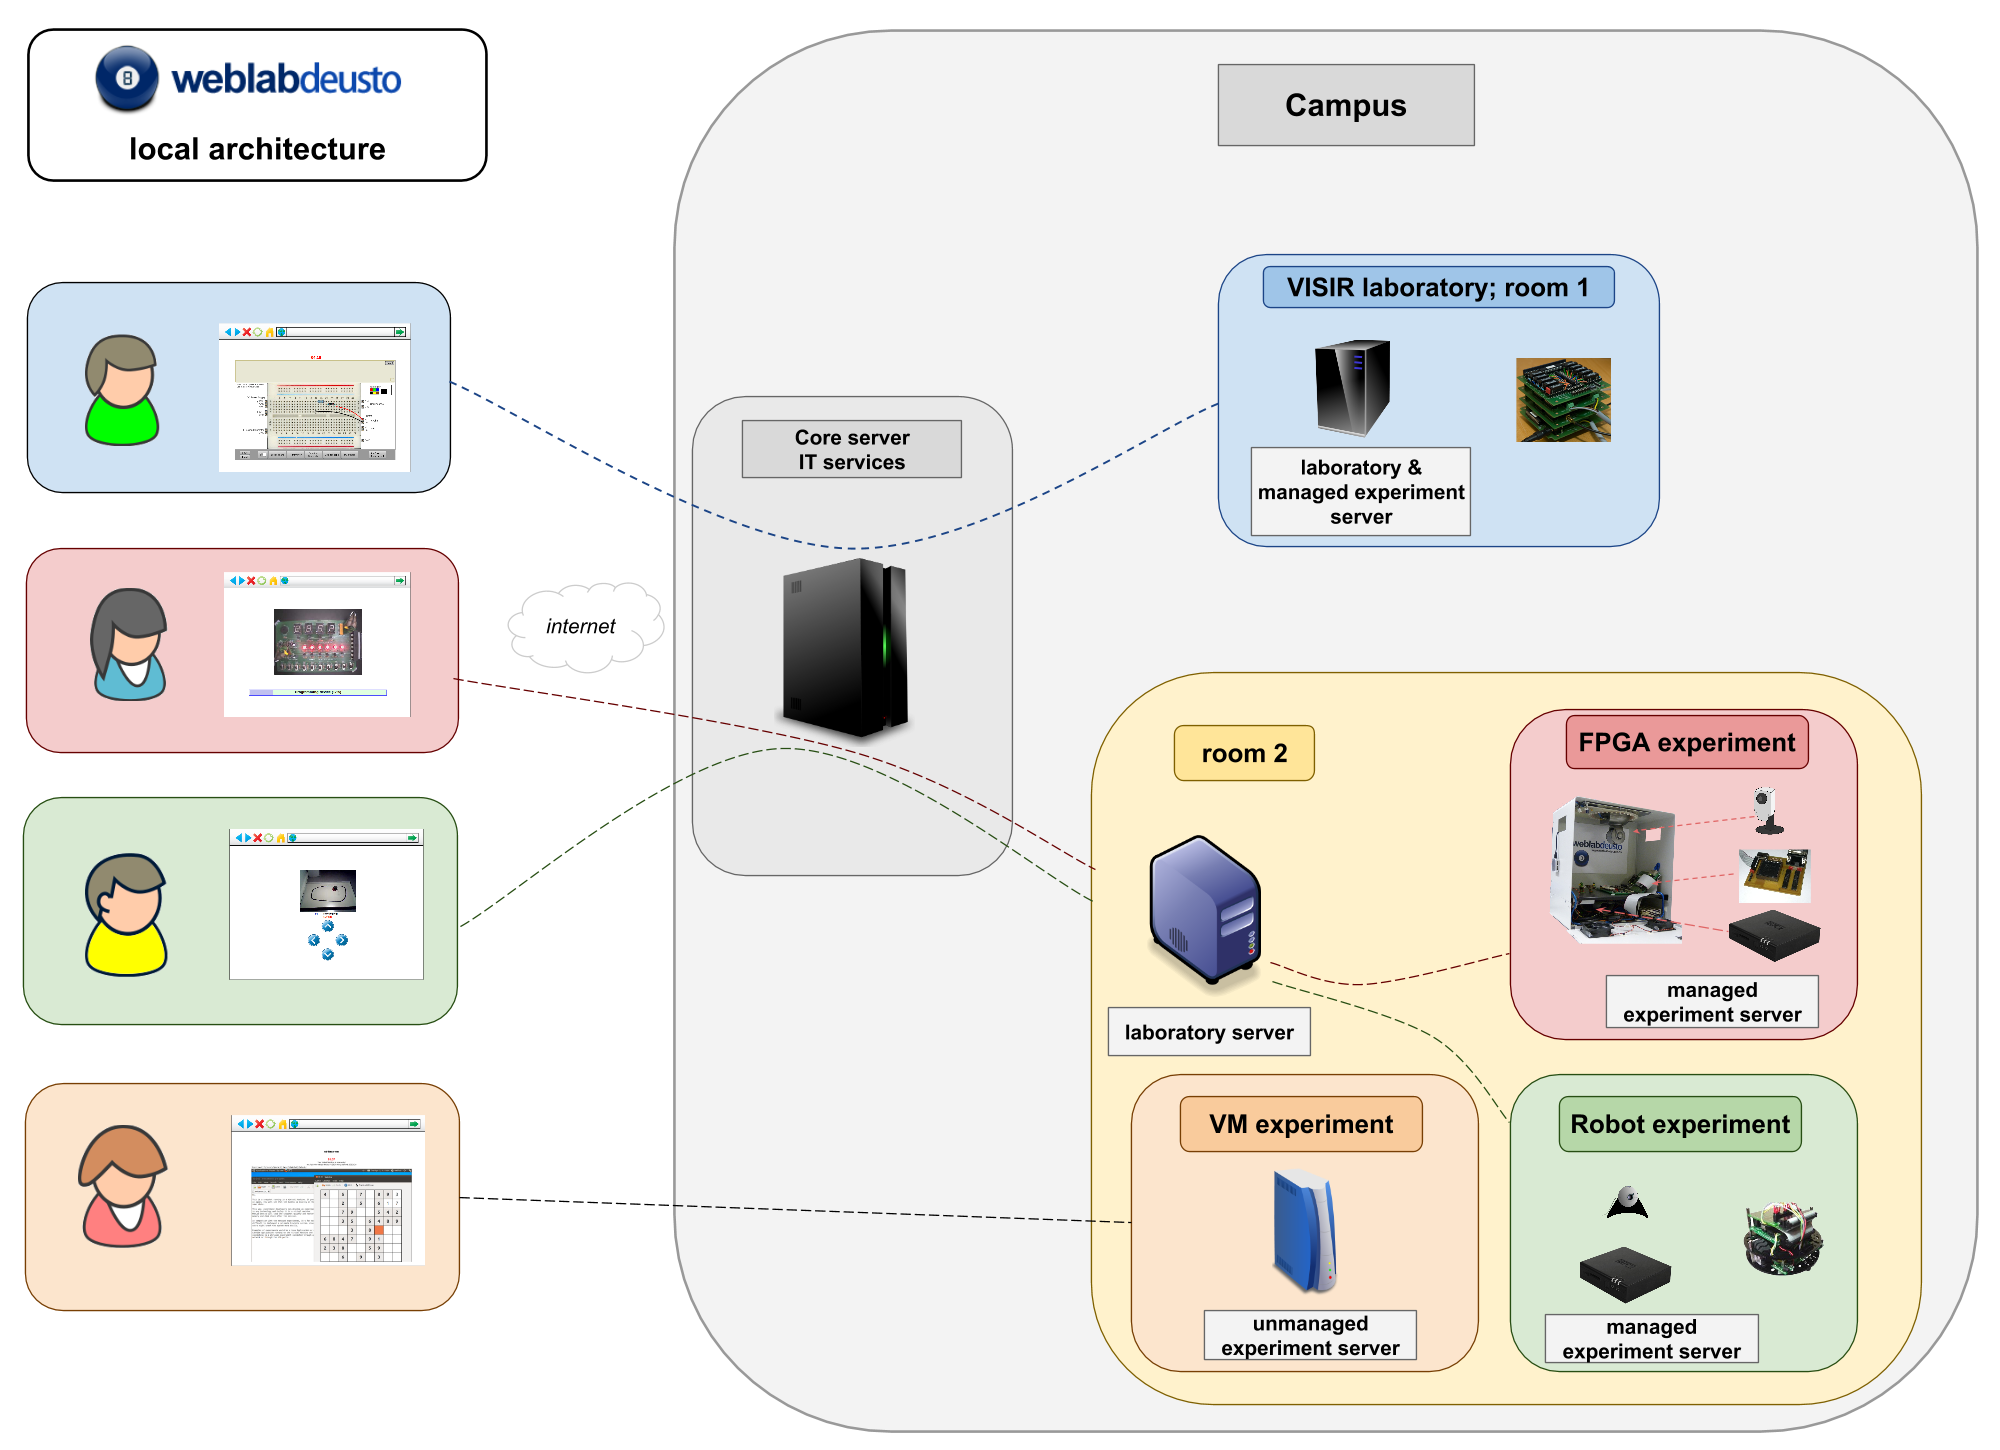
\includegraphics[width=0.75\textwidth]{figures/local_architecture.png}
    \caption{Arquitectura \textit{WebLab-Deusto}}
    \label{fig:arquitecturawld}
\end{figure}

Nesta tipo de arquitectura, os utilizadores(clientes) ligam-se aos servidores principais e estes gerem a autenticação, a autorização, o controlo dos utilizadores, etc.
Suporta nativamente a ``Federação'' de \acrshort{laboratório remoto}s, o que significa que se duas universidades instalarem o \textit{WebLab-Deusto}, qualquer um dos sistemas poderá usar os laboratórios fornecidos pela outra universidade.
Além disso, fornece bibliotecas tanto do lado do cliente, como do lado do servidor para lidar com as comunicações e também fornece componentes de \textit{software} que estarão entre cliente e servidor \cite{wlddoc}.

A gateways4labs\footnote{https://gateway4labs.readthedocs.io/en/latest/} é, também, uma abordagem \textit{open-source} que visa a integração de múltiplos laboratórios remotos em diferentes ambientes de aprendizagem digital (ferramentas digitais) através de uma \textit{interface} única.
A arquitectura do \textit{gateway4labs} está representada na Figura \ref{fig:arqgateway4labs}. O lado esquerdo - denominado o ``lado do cliente'' - contém ferramentas de aprendizagem, como por exemplo o \textit{moodle}. O lado direito - denominado o ``lado do laboratório'' - representa o \acrshort{rlms}, por exemplo, um dos dois casos abordados anteriormente: \textit{WebLab-Deusto} ou \acrshort{ilab}\cite{Orduñag4l}.
A parte central, \textit{LabManager}, é responsável pela recepção dos vários pedidos de diferentes \acrfull{lms}s(que é o local onde os alunos e os professores se encontram e onde os alunos encontram outros recursos educativos) e compreenderá os protocolos de diferentes \acrshort{rlms}s, não tendo qualquer código dependente dos \acrshort{lms}s, mas dispondo de \textit{plug-ins} dependentes de \acrshort{rlms}s\cite{Orduñag4l}\cite{g4ldocumentation}.
\begin{figure}[hbtp]
    \centering
    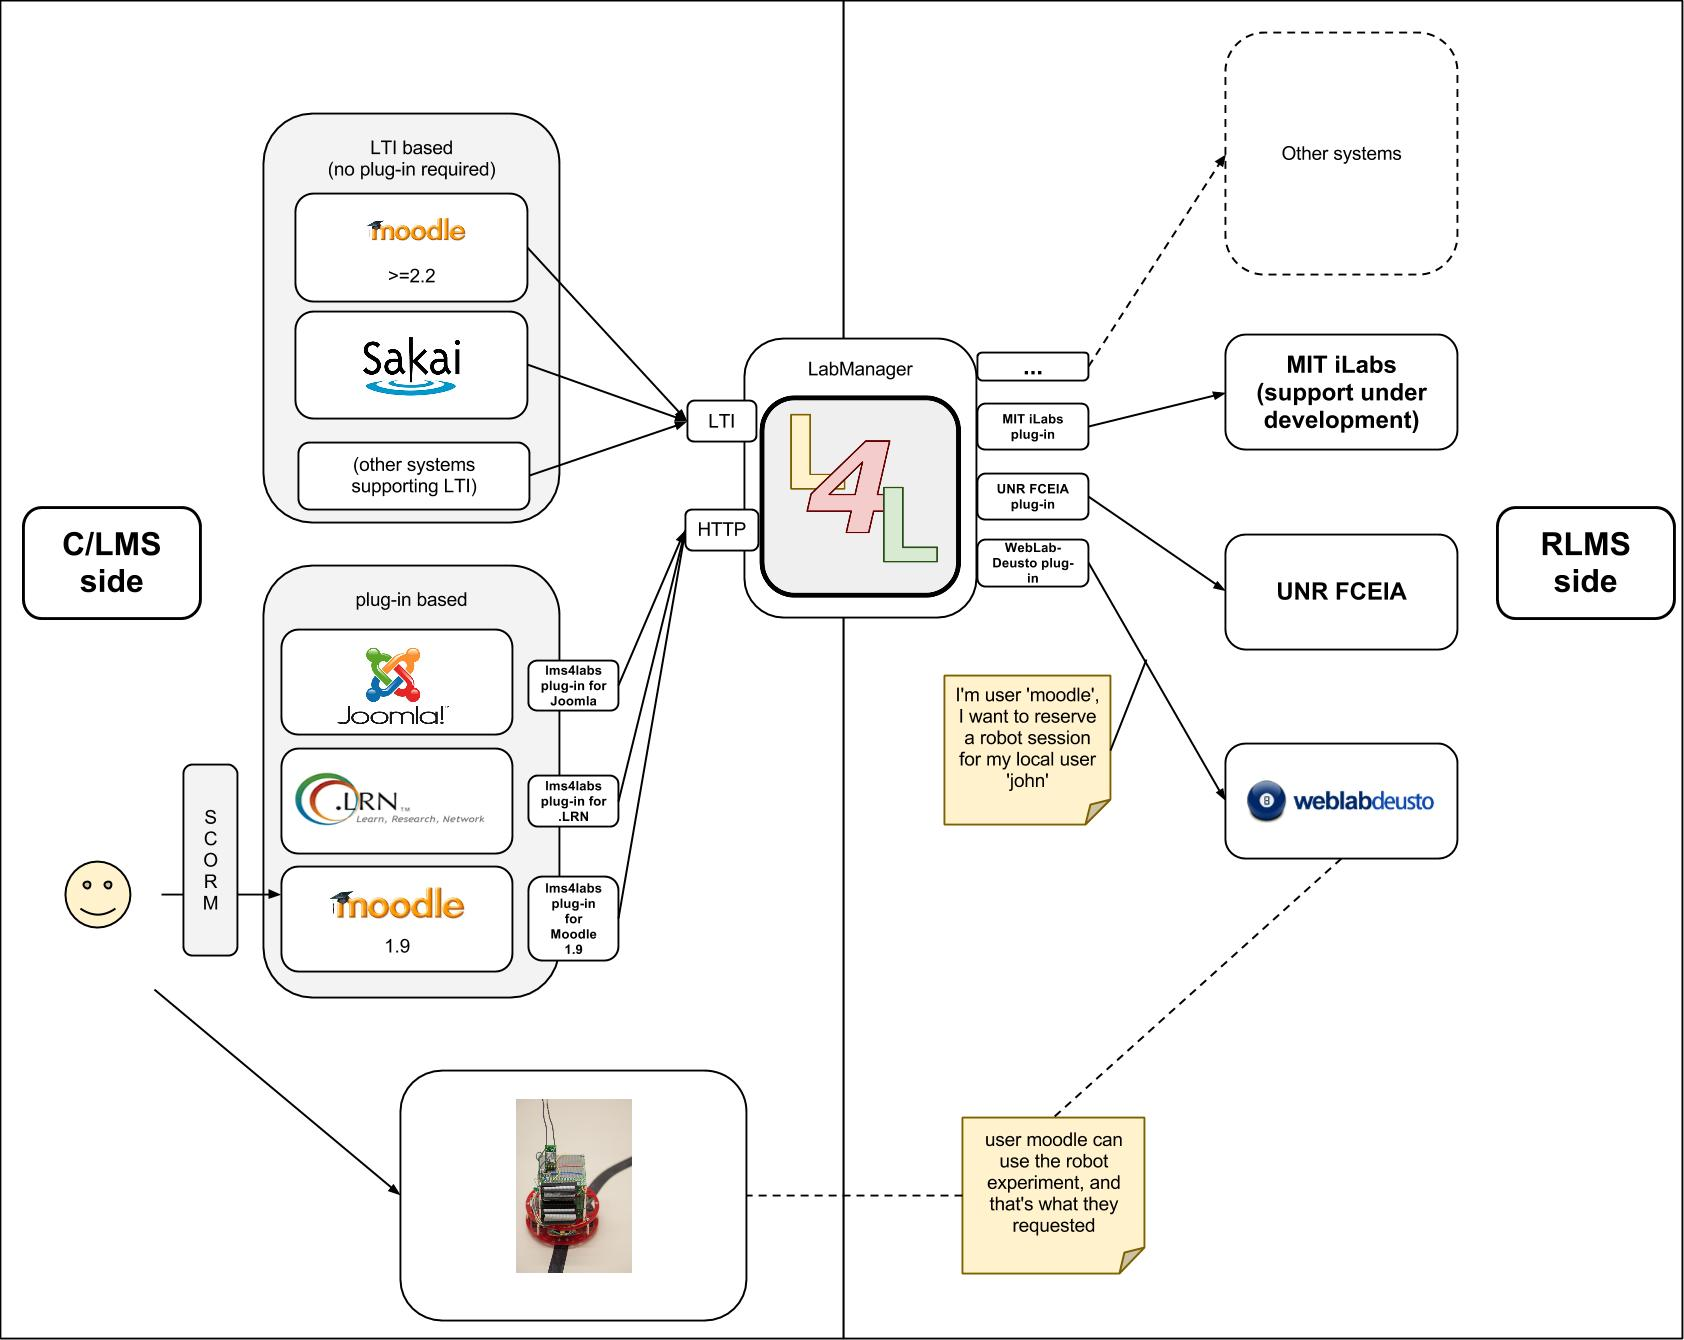
\includegraphics[width=0.8\textwidth]{figures/g4l_general_architecture.png}
    \caption{Arquitectura \textit{gateway4labs}}
    \label{fig:arqgateway4labs}
\end{figure}

Uma derivação do \textit{WebLab-Deusto} é o \textit{LabsLand}\footnote{\url{https://labsland.com/}} que interliga escolas e universidades com laboratórios reais disponíveis noutro local\footnote{\url{https://developers.labsland.com/weblablib/en/stable/}}. Fornece um repositório de laboratórios remotos de diferentes instituições ligados entre si. Também presta serviços de consultoria e vende laboratórios remotos\footnote{\url{https://weblab.deusto.es/website/index.html}}.

Outra forma de integrar \acrshort{laboratório remoto}s - nomeadamente, o \acrshort{visir} - é o sistema \textit{Maxwell}\footnote{\url{https://www.maxwell.vrac.puc-rio.br/}}, desenvolvido e integrado na \acrfull{puc} - Rio, Rio de Janeiro\footnote{\url{https://www.puc-rio.br/index.html}}. A \acrshort{puc} - Rio, possui um \acrshort{lms} integrado num repositório institucional e o \acrshort{visir}, assim como o \acrshort{labview}, podem ser utilizado a partir do \acrshort{lms}. Os alunos acedem ao \acrshort{laboratório remoto} através do \textit{weblab}\cite{Alves}.

\textbf{- Desenvolver um pouco mais o conceito de ``FEDERAÇÃO'' - PROF??}

\paragraph{VISIR}
\label{sec:visir}
No contexto desta dissertação, importa abordar o caso mais particular do \acrshort{visir}. De facto, este \acrshort{laboratório remoto} esteve na génese da criação do \acrshort{lare}. Além do mais, está disponível no \acrshort{isep}, Figura \ref{fig:visirISEP}. Como já foi referido, o \acrshort{visir} também se encontra implementado na Universidade de Deusto, mais concretamente, como parte integrante do \textit{WebLab-Deusto}.

\begin{figure}[hbtp]
    \centering
    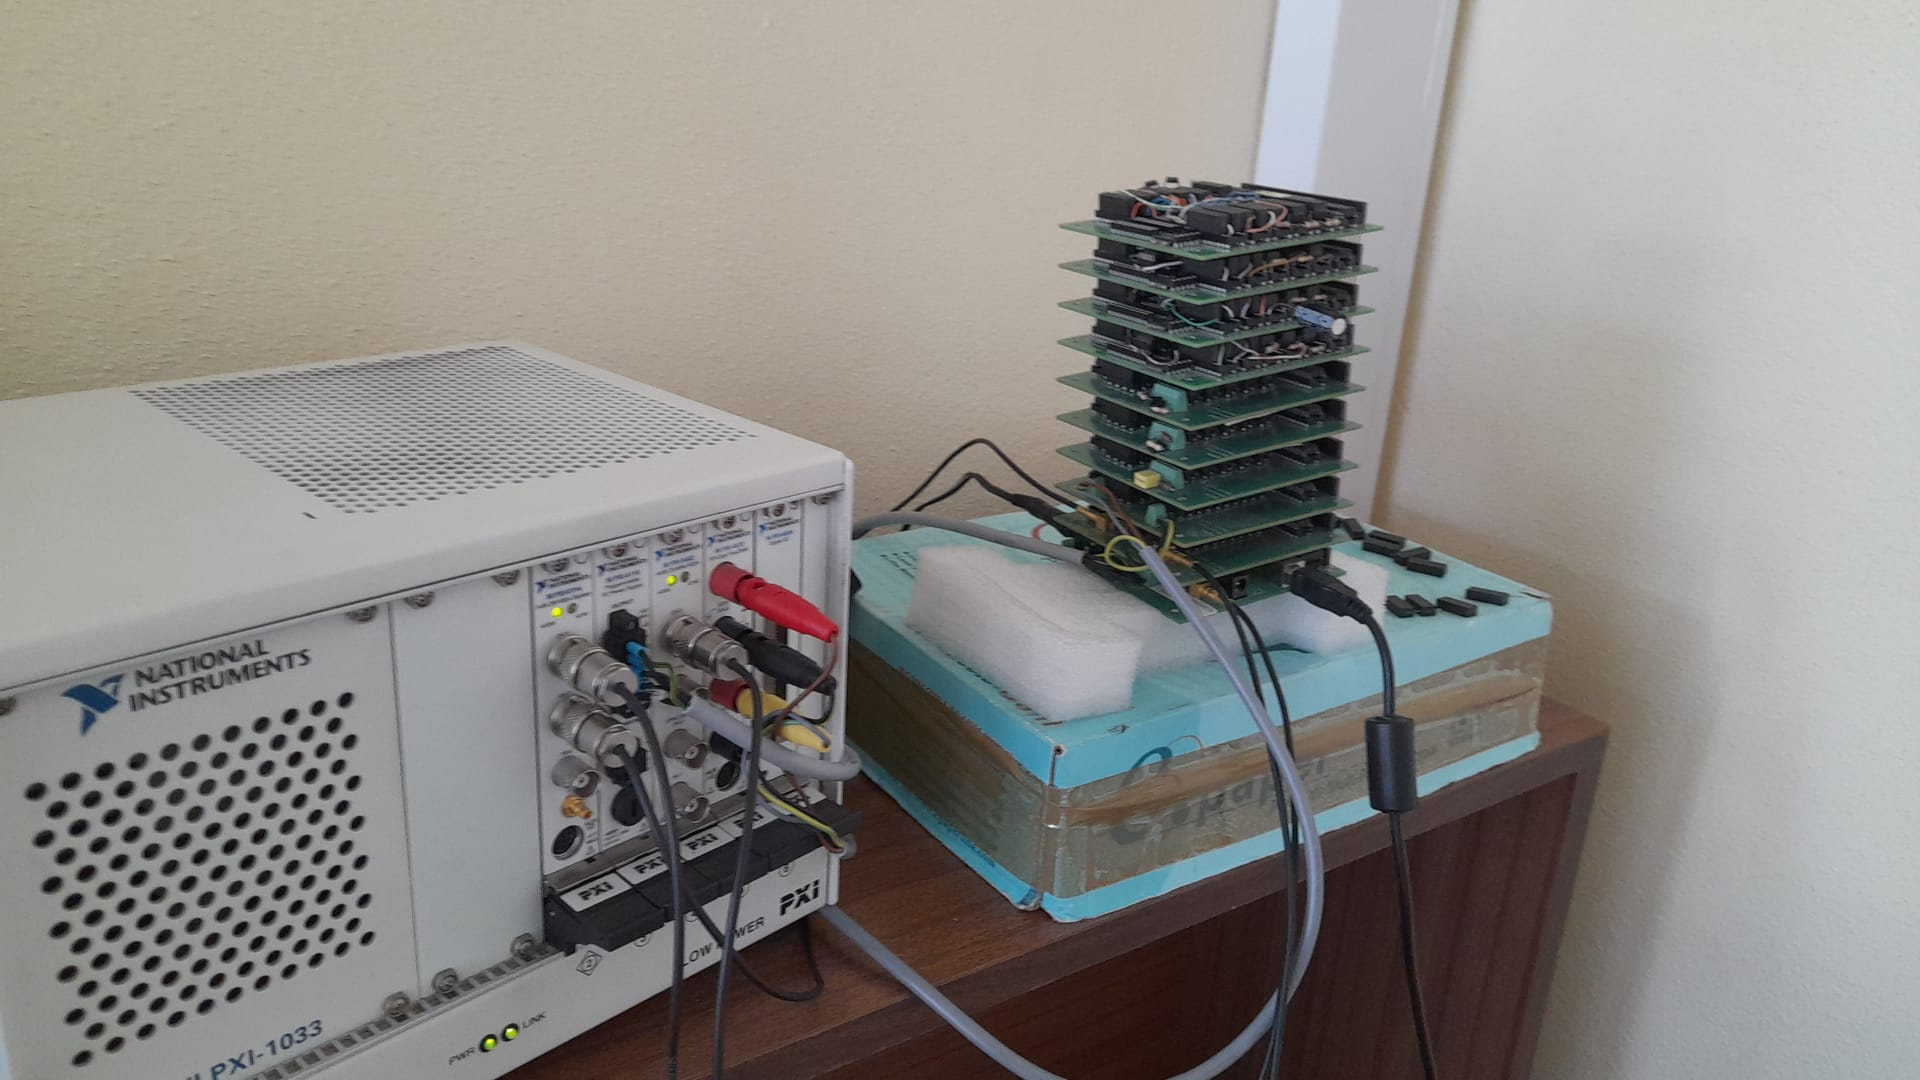
\includegraphics[width=0.75\textwidth]{figures/visirISEP.jpeg}
    \caption{\acrshort{visir} no \acrshort{isep}}
    \label{fig:visirISEP}
\end{figure}

O \acrshort{visir} é um \acrshort{laboratório remoto} para concepção, ligação e medição de circuitos electrónicos. O sistema \acrshort{visir} foi desenvolvido no \acrfull{bth}, \textit{Karlskrona}, Suécia, em 1999, e as suas funcionalidades e comunidade de utilizadores têm vindo a crescer desde então \cite{RemoteLabsImpactVISIR}. O projecto foi lançado no final de 2006 em conjunto com a \acrshort{ni}, nos \acrshort{eua}, (como fornecedor de instrumentos) e a \textit{Axiom EduTECH} na Suécia (como fornecedor de educação, \textit{software} técnico e serviços de engenharia para análise de ruído e vibrações). Foi apoiado financeiramente pela \acrshort{bth} e pela Agência Governamental Sueca para os Sistemas de Inovação (VINNOVA)\cite{VISIRExperiencesChallenges}.

O \acrshort{visir} oferece aos estudantes a oportunidade de utilizarem recursos experimentais gratuitos 24 horas por dia, 7 dias por semana, sem um aumento significativo no custo por estudante. Com mais tempo dedicado a estas experiências, os estudantes tornam-se verdadeiros ''experimentadores``, capazes de criar bens e serviços que satisfaçam os requisitos de uma sociedade sustentável. Desta forma, o \acrshort{visir} não só melhora a aprendizagem, mas também contribui para a formação de profissionais comprometidos com o desenvolvimento sustentável \cite{OpenLabs77:online}.

Em 2018, tal como referido em \cite{PILARFederationVISIR}, o \acrshort{visir} já tinha sido implementado em 8 Instituições de Ensino Superior diferentes, situados em 6 países, incluindo o \acrshort{isep} (Portugal). No mesmo ano, segundo a mesma publicação, foram instalados novos sistemas \acrshort{visir} em várias instituições da América do Sul. O software do \acrshort{visir} é lançado sob uma licença GNU GPL.

O conceito subjacente a este consiste em acrescentar uma opção de operação remota aos laboratórios de ensino tradicionais para os tornar mais acessíveis, independentemente dos alunos estarem no \textit{campus} ou principalmente fora do \textit{campus}\cite{TheVISIRproject}.

A arquitectura, do \acrshort{visir} pode ser dividida em quatro partes, tal como referido em \cite{tawfikexperiences} e como se pode ver na Figura \ref{fig:arquitecturavisir} esta arquitectura inclui:
\begin{itemize}
    \item Servidor de equipamento - Compreende todo o equipamento do \acrshort{visir} (módulos e \textit{chassis}): as placas \acrfull{pxi} e instrumentação (que estão ligadas à matriz de relés) controlados através do \acrshort{labview};
    \item Servidor de medições - Trata-se de um servidor escrito em Visual C++ para a \textit{Microsoft}. É programado por ficheiros ``max list'' que contêm os valores máximos dos componentes e ajustes dos instrumentos para cada experiência e servem para evitar a concepção de circuitos perigosos e proteger os instrumentos;
    \item Servidor \textit{web} - Aloja a \textit{interface Web} do \acrshort{visir} e foi concebida em \textit{Apache} com uma base de dados em \textit{MySQL};
    \item Servidor de \textit{interface}, Figura \ref{fig:protboard_visir} - É o \textit{site} do \acrshort{visir} e foi escrito em PHP, com o cliente de experiências integrado escrito em \textit{Flash}.
\end{itemize}

\begin{figure}[hbtp]
    \centering
    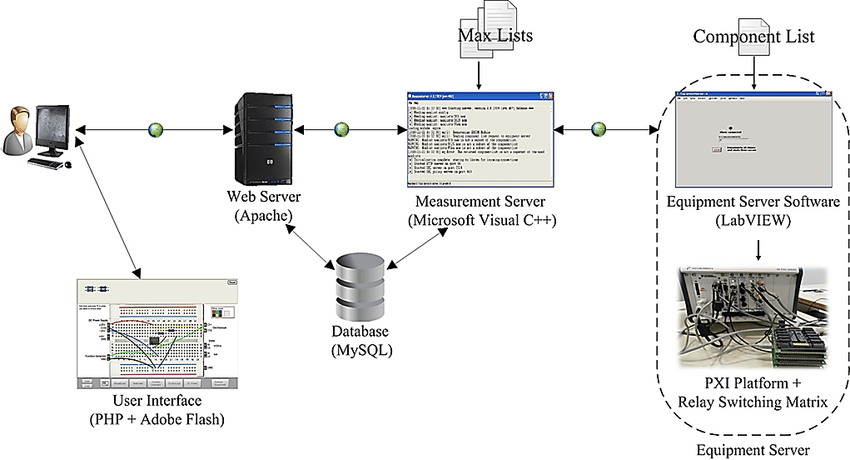
\includegraphics[width=0.75\textwidth]{figures/arquitectura_VISIR.png}
    \caption{Arquitectura \acrshort{visir}\cite{tawfikexperiences}}
    \label{fig:arquitecturavisir}
\end{figure}

\begin{figure}[hbtp]
    \centering
    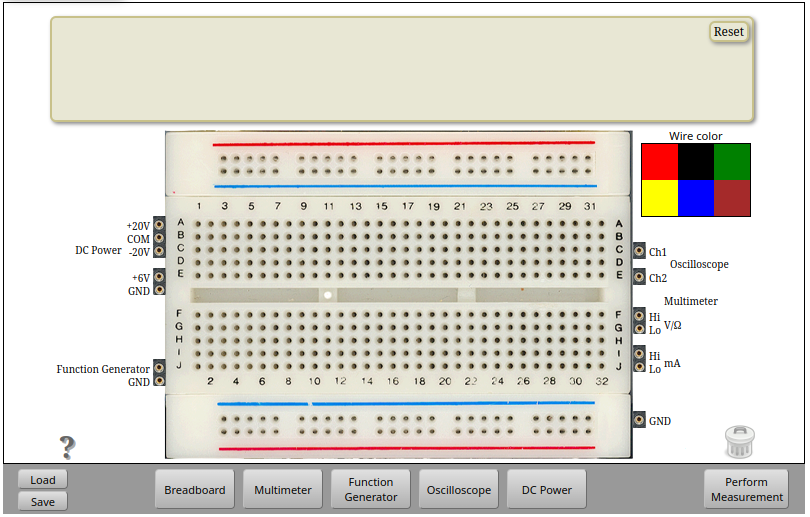
\includegraphics[width=0.75\linewidth]{figures/protboard_visir.png}
    \caption{\textit{Protobaord \acrshort{visir}}}
    \label{fig:protboard_visir}
\end{figure}

O \textit{chassis}  PXI-1033\cite{PXI-1033}, Figura \ref{fig:PXI-1033}, é um controlador integrado com 5 \textit{slots} que foi concebida para aplicações de controlo remoto. Obviamente que esta placa exige um \textit{interface} para \acrshort{pc}, que, neste caso, é feito através do \acrshort{labview}.

\begin{figure}[hbtp]
    \centering
    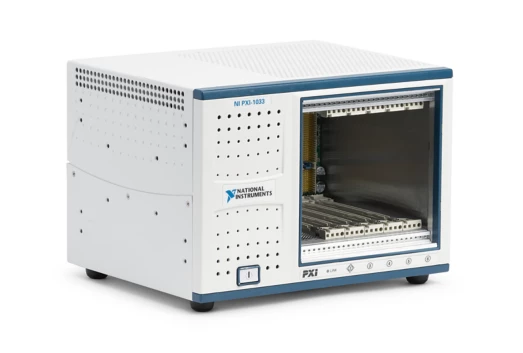
\includegraphics[width=0.75\textwidth]{figures/PXI-1033.png}
    \caption{\textit{Chassis} PXI-1033 \cite{PXI-1033}}
    \label{fig:PXI-1033}
\end{figure}

Os módulos integrados na PXI-1033 e que compõem o \acrshort{visir} são:
\begin{itemize}
    \item Osciloscópio, PXI-5114, \SI{12}{\MHz}, 250 MS/s, 8-Bit, Figura \ref{fig:PXI-5114}
          \begin{figure}[hbtp]
              \centering
              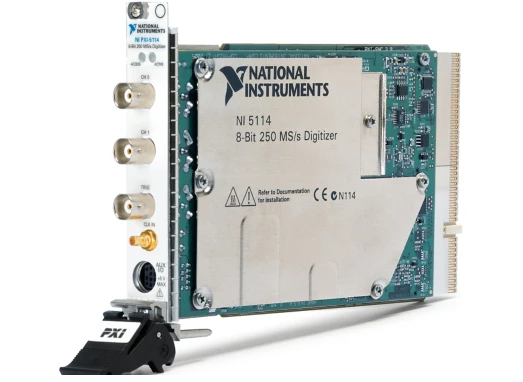
\includegraphics[width=0.75\textwidth]{figures/PXI-5114.png}
              \caption{Osciloscópio PXI-5114 \cite{PXI-5114}}
              \label{fig:PXI-5114}
          \end{figure}
    \item Gerador de sinal, PXI-5402, \SI{10}{\MHz} \textit{Bandwidth}, 1-\textit{Channel}, 14-Bit, Figura \ref{fig:PXI-5402}
          \begin{figure}[hbtp]
              \centering
              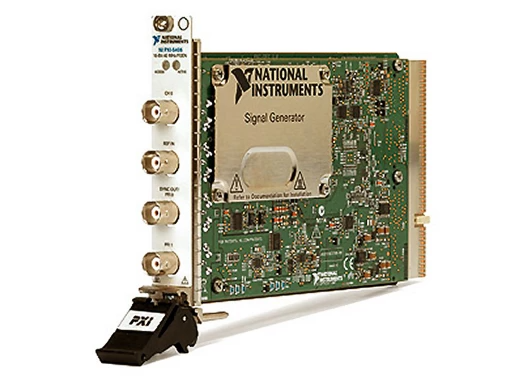
\includegraphics[width=0.75\textwidth]{figures/PXI-5402.png}
              \caption{Gerador de sinal PXI-5402 \cite{PXI-5402}}
              \label{fig:PXI-5402}
          \end{figure}
    \item Multímetro Digital, \(6^{1/2} \)Digitos, \(\pm\)\SI{300}{\volt}, \textit{Onboard} 1.8 MS/s Digitalizador isolado, suporte para medições de indutâncias e capacitâncias, Figura \ref{fig:PXI-4072};
          \begin{figure}[hbtp]
              \centering
              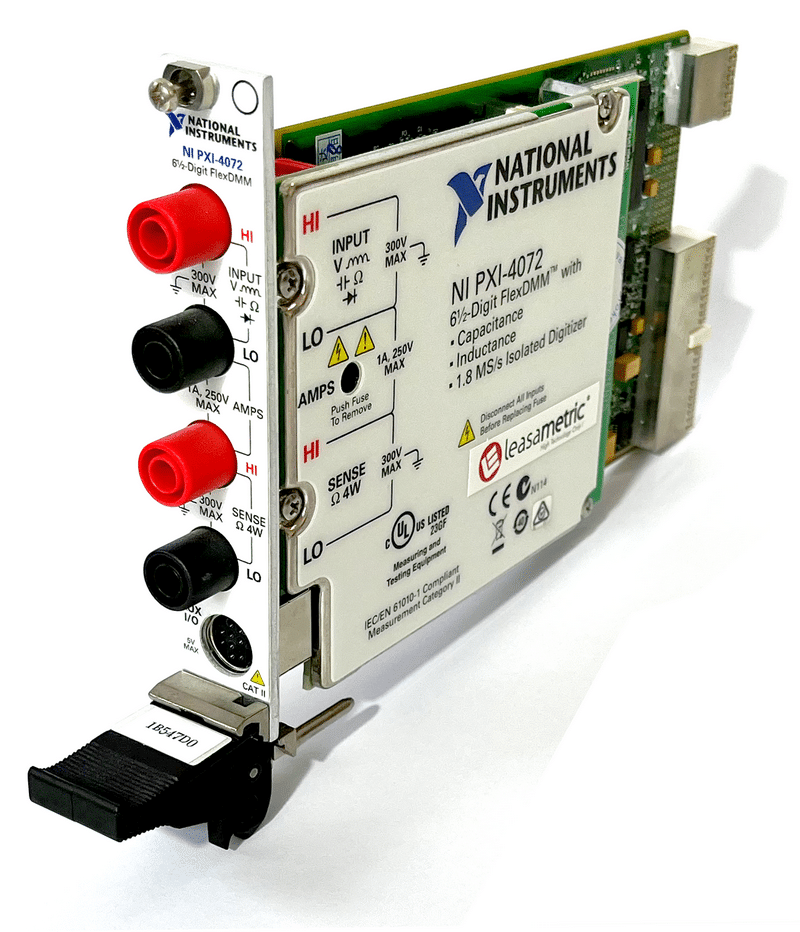
\includegraphics[width=0.6\textwidth]{figures/PXI-4072.png}
              \caption{Multímetro Digital PXI-4072 \cite{PXI-4072}}
              \label{fig:PXI-4072}
          \end{figure}
    \item Fonte de tensão programável, 3 canais, corrente de saída máxima de \SI{1}{\ampere}, gama de tensão de saída analógica: -\SI{20}{\volt} a \SI{20}{\volt}, Figura {\ref{fig:PXI-4110}}.
          \begin{figure}[hbtp]
              \centering
              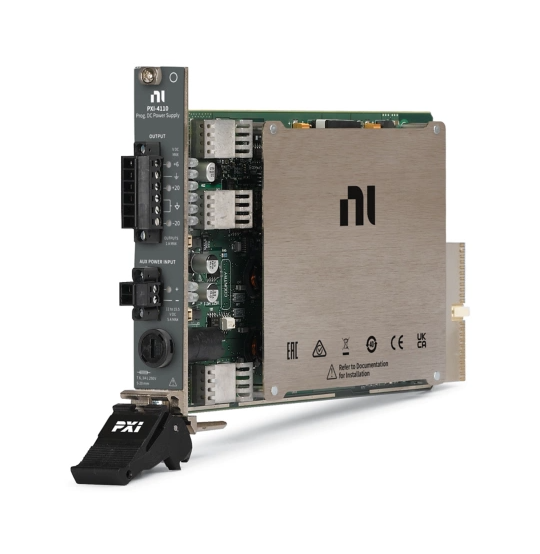
\includegraphics[width=0.7\textwidth]{figures/PXI-4110.png}
              \caption{Fonte de tensão PXI-4110 \cite{PXI-4110}}
              \label{fig:PXI-4110}
          \end{figure}
\end{itemize}

O \acrshort{visir} possuí uma \acrfull{mcr} concebida no \acrshort{bth} especialmente para o uso em experiências electrónicas em \acrshort{laboratório remoto}s, Figura \ref{fig:matrizvisir}. Esta matriz é constituída por quatro placas PC/104\footnote{\url{https://pc104.org/}} (de baixo para cima): \textbf{NOTA: subentende-se que são placas de controlo - A REVER} fontes de tensão, multímetro digital, osciloscópio e a placa de topo permite configurar os componentes. A matriz é controlada por uma \acrfull{pic}, \\PIC18F4550\footnote{\textit{Datasheet}: \url{https://www.microchip.com/en-us/product/PIC18F4550}}, montada na placa de alimentação (fontes de tensão) e comunica com um \acrshort{pc}, via \acrshort{usb}, e com os controladores das outras placas através das \acrshort{pic}s, PIC16F767\footnote{\textit{Datasheet}: \url{https://www.microchip.com/en-us/product/PIC16F767}}, via \acrfull{i2c}, montadas em cada placa\cite{matriz}.

\begin{figure}[hbtp]
    \centering
    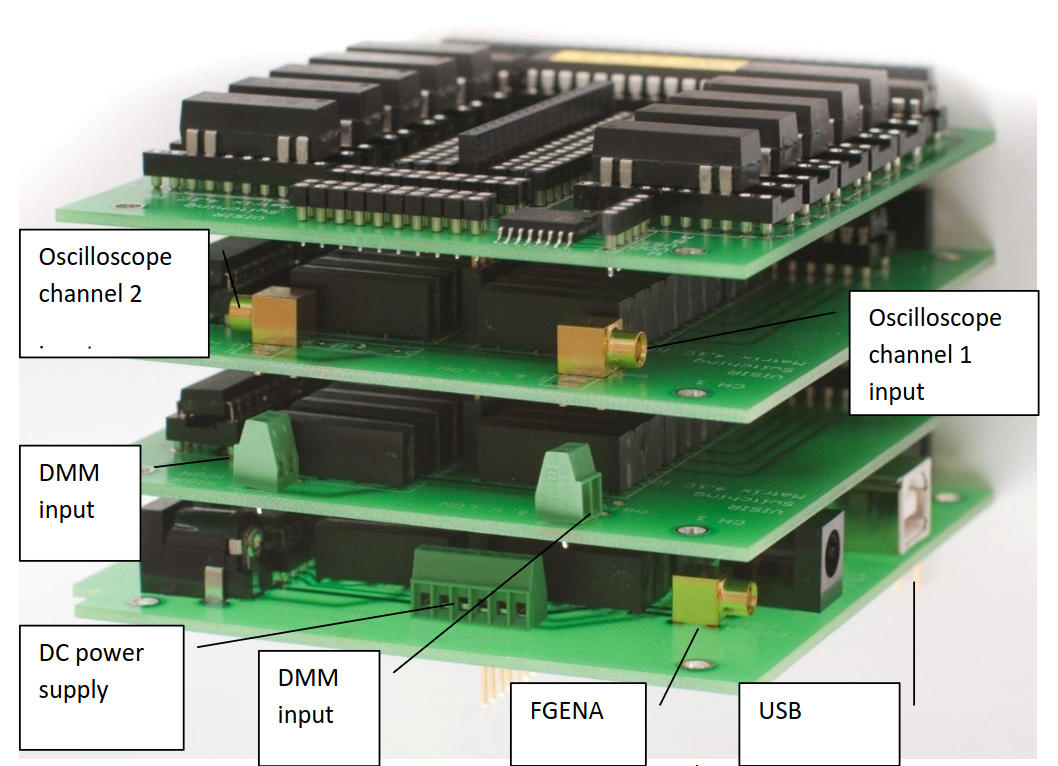
\includegraphics[width=0.7\textwidth]{figures/matriz.png}
    \caption{Matriz \acrshort{visir}\cite{matriz}}
    \label{fig:matrizvisir}
\end{figure}

Segundo \cite{tawfikexperiences} e \cite{tawfikvisir}, em 2012, 6 Universidades tinham implementado o \acrshort{visir}. No entanto, Pereira \textit{et all.}, (2017), referem que o \acrshort{visir} estava presente em 12 instituições e 7 países\cite{pereira}.

\vspace{0.5cm}
Levanta-se, então, uma questão: Como fazer a integração de todos os \acrshort{laboratório remoto}s de forma a aproveitar os recursos e potenciar o trabalho colaborativo?
\vspace{0.5cm}

\paragraph{PILAR}
O projecto \textbf{\acrfull{pilar}} \textit{Erasums+}, foi iniciado em 2016 tendo terminado em 2019 e tinha como objectivo a criação de uma Federação de cinco nós \acrshort{visir} existentes, partilhando experiências, capacidade e recursos entre as diversas instituições e permitir o acesso ao \acrshort{laboratório remoto} \acrshort{visir}, através do consórcio \acrshort{pilar}, a estudantes de outras instituições de ensino\cite{garcia-loro}.

O \acrshort{visir} \acrfull{sig} é(\textbf{FOI - A REVER PROF}) organizado para pessoas interessadas em Engenharia \textit{online} ou remota, especialmente na abertura de laboratórios universitários para acesso remoto 24/7. Este projeto foi lançado com o objetivo de divulgar métodos de abertura de laboratórios para acesso remoto,  partilhar ideias, equipamento e material didático, bem como de discutir o desenvolvimento da plataforma \acrshort{visir}. Outro dos objetivos é(\textbf{FOI - A REVER PROF}) a padronização de bancos de trabalho \textit{online} localizados em universidades de todo o mundo, constituindo laboratórios de rede disponíveis para sessões de laboratório para estudantes dentro e fora do \textit{campus}\cite{visirsig}.

A missão da Federação \acrshort{visir} é actualizar e alargar o \acrshort{visir} \acrshort{sig}, integrando indivíduos e instituições. O objetivo é fornecer um sistema uniforme, em que os estudantes se possam registar e utilizar os laboratórios federados baseados no \acrshort{visir} e os materiais de aprendizagem de diferentes instituições pertencentes à Federação. Através de um mecanismo comum partilhado, deverá ser possível aceder a cada experiência a partir de um único sistema de gestão da aprendizagem \cite{visirfederation}.

Os principais objectivos da Federação são\cite{visirfederation}:
\begin{itemize}
    \item Expandir o \acrshort{sig} a instituições;
    \item Conectar todos os nós \acrshort{visir};
    \item Alargar a gama de aplicações;
    \item Melhorar a utilização do \acrshort{visir};
    \item Promover o laboratório remoto \acrshort{visir};
    \item Partilhar materiais de aprendizagem;
    \item Trocar experiências entre os detentores e utilizadores do \acrshort{visir}.
\end{itemize}

Como se viu anteriormente, o \acrshort{visir} funciona numa base de cliente-servidor, o que significa que, se um determinado servidor não estiver disponível, também o laboratório não estará. Neste caso, a Federação permite o redireccionamento dos pedidos dos clientes para um outro nó \acrshort{visir} que esteja disponível\cite{kreiter}.

\section{COMENTÁRIO PROF}
\textbf{ Desenvolver mais o PILAR e a Federação?}

\textbf{Desenvolver mais o VISIR? Vantagens? Desafios?}